\documentclass[twoside]{book}

% Packages required by doxygen
\usepackage{fixltx2e}
\usepackage{calc}
\usepackage{doxygen}
\usepackage[export]{adjustbox} % also loads graphicx
\usepackage{graphicx}
\usepackage[utf8]{inputenc}
\usepackage{makeidx}
\usepackage{multicol}
\usepackage{multirow}
\PassOptionsToPackage{warn}{textcomp}
\usepackage{textcomp}
\usepackage[nointegrals]{wasysym}
\usepackage[table]{xcolor}

% Font selection
\usepackage[T1]{fontenc}
\usepackage[scaled=.90]{helvet}
\usepackage{courier}
\usepackage{amssymb}
\usepackage{sectsty}
\renewcommand{\familydefault}{\sfdefault}
\allsectionsfont{%
  \fontseries{bc}\selectfont%
  \color{darkgray}%
}
\renewcommand{\DoxyLabelFont}{%
  \fontseries{bc}\selectfont%
  \color{darkgray}%
}
\newcommand{\+}{\discretionary{\mbox{\scriptsize$\hookleftarrow$}}{}{}}

% Page & text layout
\usepackage{geometry}
\geometry{%
  a4paper,%
  top=2.5cm,%
  bottom=2.5cm,%
  left=2.5cm,%
  right=2.5cm%
}
\tolerance=750
\hfuzz=15pt
\hbadness=750
\setlength{\emergencystretch}{15pt}
\setlength{\parindent}{0cm}
\setlength{\parskip}{3ex plus 2ex minus 2ex}
\makeatletter
\renewcommand{\paragraph}{%
  \@startsection{paragraph}{4}{0ex}{-1.0ex}{1.0ex}{%
    \normalfont\normalsize\bfseries\SS@parafont%
  }%
}
\renewcommand{\subparagraph}{%
  \@startsection{subparagraph}{5}{0ex}{-1.0ex}{1.0ex}{%
    \normalfont\normalsize\bfseries\SS@subparafont%
  }%
}
\makeatother

% Headers & footers
\usepackage{fancyhdr}
\pagestyle{fancyplain}
\fancyhead[LE]{\fancyplain{}{\bfseries\thepage}}
\fancyhead[CE]{\fancyplain{}{}}
\fancyhead[RE]{\fancyplain{}{\bfseries\leftmark}}
\fancyhead[LO]{\fancyplain{}{\bfseries\rightmark}}
\fancyhead[CO]{\fancyplain{}{}}
\fancyhead[RO]{\fancyplain{}{\bfseries\thepage}}
\fancyfoot[LE]{\fancyplain{}{}}
\fancyfoot[CE]{\fancyplain{}{}}
\fancyfoot[RE]{\fancyplain{}{\bfseries\scriptsize Generated by Doxygen }}
\fancyfoot[LO]{\fancyplain{}{\bfseries\scriptsize Generated by Doxygen }}
\fancyfoot[CO]{\fancyplain{}{}}
\fancyfoot[RO]{\fancyplain{}{}}
\renewcommand{\footrulewidth}{0.4pt}
\renewcommand{\chaptermark}[1]{%
  \markboth{#1}{}%
}
\renewcommand{\sectionmark}[1]{%
  \markright{\thesection\ #1}%
}

% Indices & bibliography
\usepackage{natbib}
\usepackage[titles]{tocloft}
\setcounter{tocdepth}{3}
\setcounter{secnumdepth}{5}
\makeindex

% Hyperlinks (required, but should be loaded last)
\usepackage{ifpdf}
\ifpdf
  \usepackage[pdftex,pagebackref=true]{hyperref}
\else
  \usepackage[ps2pdf,pagebackref=true]{hyperref}
\fi
\hypersetup{%
  colorlinks=true,%
  linkcolor=blue,%
  citecolor=blue,%
  unicode%
}

% Custom commands
\newcommand{\clearemptydoublepage}{%
  \newpage{\pagestyle{empty}\cleardoublepage}%
}

\usepackage{caption}
\captionsetup{labelsep=space,justification=centering,font={bf},singlelinecheck=off,skip=4pt,position=top}

%===== C O N T E N T S =====

\begin{document}

% Titlepage & ToC
\hypersetup{pageanchor=false,
             bookmarksnumbered=true,
             pdfencoding=unicode
            }
\pagenumbering{alph}
\begin{titlepage}
\vspace*{7cm}
\begin{center}%
{\Large Project9-\/\+Monte-\/\+Carlo \\[1ex]\large 1.\+0 }\\
\vspace*{1cm}
{\large Generated by Doxygen 1.8.13}\\
\end{center}
\end{titlepage}
\clearemptydoublepage
\pagenumbering{roman}
\tableofcontents
\clearemptydoublepage
\pagenumbering{arabic}
\hypersetup{pageanchor=true}

%--- Begin generated contents ---
\chapter{Monte Carlo}
\label{index}\hypertarget{index}{}\subsubsection*{Authors \+:}

Akeddar Mehdi 261344

Birch Hugo 261684

\subsubsection*{Description}

This project is an introduction to scientific programming in C ++. It is registered as part of the Programming Concepts in Scientific Computing course(\href{https://edu.epfl.ch/coursebook/fr/programming-concepts-in-scientific-computing-MATH-458}{\tt https\+://edu.\+epfl.\+ch/coursebook/fr/programming-\/concepts-\/in-\/scientific-\/computing-\/\+M\+A\+T\+H-\/458}).

The objective of the project is the creation of a Monte Carlo algorithm in a modular way. To do this, the following objectives have been achieved \+:
\begin{DoxyItemize}
\item Implementation of random number generators with a normal \& uniform probability distribution.
\item The compute of the expectation value of a user-\/defined function
\item The visualization of the statistical moments
\item The graphical verification of Central Limit Theorem (C\+TL)
\end{DoxyItemize}

\subsubsection*{How It Works}

To run the executable, the following information must be written to the terminal \+:

\textquotesingle{}./project9 name\+\_\+of\+\_\+distribution\+\_\+file name\+\_\+of\+\_\+function\+\_\+file distribution type\textquotesingle{} .

The program returns an output directory containing a \textquotesingle{}moments.\+csv\textquotesingle{} file with moment results and several \textquotesingle{}sample\+\_\+means.\+csv\textquotesingle{} to verify the C\+TL theorem.

If run in C\+Lion I\+DE the arguments are saved to run with the default files to allow to be run directly\+:
\begin{DoxyItemize}
\item test\+\_\+function.\+txt
\item test\+\_\+normal.\+txt
\item \textquotesingle{}N\textquotesingle{} as distribution type.
\end{DoxyItemize}

To plot the results, the \textquotesingle{}visualization.\+py\textquotesingle{} script should be run. It ouputs 3 graphs \+: A visualization of the moments, 2 visualizations of the C\+TL theorem \+: The normal distribution of the sample means and the value of the sample\textquotesingle{}s standard distribution compared to the theoretical standard distribution.

\subsubsection*{Input files}

2 input files are needed for code usage \+:
\begin{DoxyItemize}
\item A Distribution file \+: the file should be structured as follow \+:
\begin{DoxyItemize}
\item The size of the vector.
\item The mean of the normal distribution or the lower bound of the uniform distribution.
\item The variance of the distribution or the upper bound of the uniform distribution.
\end{DoxyItemize}
\item A Function file \+: the file should be structured as follow \+:
\begin{DoxyItemize}
\item The type of function \+: \textquotesingle{} P \textquotesingle{} for polynomial, \textquotesingle{}E\textquotesingle{} for exponential and \textquotesingle{}T\textquotesingle{} for trigonometric function
\item The first coefficient \+: {\bfseries a$\ast$$\ast$x+b / $\ast$$\ast$a} exp(bx) / {\bfseries a$\ast$$\ast$cos(bx)}
\item {\bfseries The second coefficient \+: ax+$\ast$$\ast$b} / a exp($<$strong$>$b$\ast$$\ast$x) / acos($\ast$$\ast$b$\ast$$\ast$x)
\item The maximum order for the statistical moments. This code is designed for $\ast$$\ast$uniform and {\bfseries normal} distributions. However, given the modularity of the code, it is easy to extend this constraint by adding new classes.
\end{DoxyItemize}
\end{DoxyItemize}

Example of input files are present in the directory as df\+\_\+function.\+txt and df\+\_\+normal.\+txt.

\subsubsection*{Prerequisites}

\paragraph*{C++}


\begin{DoxyItemize}
\item Input Files \+: Two examples are provided \textquotesingle{}test\+\_\+normal.\+txt\textquotesingle{} and \textquotesingle{}test\+\_\+function.\+txt\textquotesingle{}. If missing input files, the code exit with an error.
\item This version was designed for C++ 14 or higher.
\item No external libraries are required. \paragraph*{Python}
\end{DoxyItemize}


\begin{DoxyItemize}
\item This version was designed for Python 3.\+6 or higher.
\item A directory called \textquotesingle{}output\textquotesingle{} containing the results for the moments and the C\+TL theorem is needed to run the visualization.
\end{DoxyItemize}

\subsubsection*{Google Test}

This project possesses 5 unit test programs\+:
\begin{DoxyItemize}
\item Reader\+\_\+test which tests that if the inputs are incorrect exceptions are thrown.
\item Normal\+Dist\+\_\+test which tests if the mean, the size and the variance given are correctly found in the normal distribution.
\item Uniform\+Dist\+\_\+test tests if the mean, the size and the variance given are correctly found in the Uniform distribution.
\item Monte\+Carlo\+Expectation\+\_\+test tests if the mean of the random sample for a uniform or normal distribution is close to the given mean. It also tests if the expectation is close to the theoretical value for both distributions.
\item Run\+All\+Tests this runs all the test described above in one go, to make it easier for the user.
\end{DoxyItemize}

All necessary Test files for the test can be found in cmake-\/build-\/debug/\+Test\+\_\+files. These unit tests are all run with the Google test library which is included in the lib directory of the Test project \subsubsection*{Doxygen}

The documentation was designed for doxygen 1.\+8.\+16 or higher. To generate the documentation, run the command \+: \textquotesingle{}doxygen Doxyfile\textquotesingle{} in the terminal.

\subsubsection*{Improvements}


\begin{DoxyEnumerate}
\item Numerous exceptions were implemented however not all cases were taken into account, so we could make the program more robust to hazardous inputs.
\item Add other type of distributions such as Poisson or Exponential.
\item Add more classes of function and more parameters to offer more possibilities of user defined functions.
\item Be more flexible on the architecture (e.\+g rethink the way readers are done to relate all readers to one abstract reader)
\item Add different way of computing the mean like a variance reduction technique.
\item Add a mathematical verification of the central limit theorem.
\end{DoxyEnumerate}

\subsubsection*{References}


\begin{DoxyItemize}
\item \href{https://en.wikipedia.org/wiki/List_of_probability_distributions}{\tt List of probability distributions}
\item \href{https://en.wikipedia.org/wiki/Normal_distribution}{\tt Normal distribution}
\item \href{https://en.wikipedia.org/wiki/Uniform_distribution_(continuous)}{\tt Uniform distribution (continuous)}
\item \href{https://en.wikipedia.org/wiki/Expected_value}{\tt Expected value}
\item \href{https://en.wikipedia.org/wiki/Central_limit_theorem}{\tt Central limit theorem}
\item \href{https://github.com/google/googletest}{\tt Google test library} 
\end{DoxyItemize}
\chapter{Hierarchical Index}
\section{Class Hierarchy}
This inheritance list is sorted roughly, but not completely, alphabetically\+:\begin{DoxyCompactList}
\item \contentsline{section}{Abstract\+Expectation}{\pageref{classAbstractExpectation}}{}
\begin{DoxyCompactList}
\item \contentsline{section}{Monte\+Carlo\+Expectation}{\pageref{classMonteCarloExpectation}}{}
\end{DoxyCompactList}
\item \contentsline{section}{Abstract\+Func}{\pageref{classAbstractFunc}}{}
\begin{DoxyCompactList}
\item \contentsline{section}{Exp\+Func}{\pageref{classExpFunc}}{}
\item \contentsline{section}{Polynom\+Func}{\pageref{classPolynomFunc}}{}
\item \contentsline{section}{Trigo\+Func}{\pageref{classTrigoFunc}}{}
\end{DoxyCompactList}
\item \contentsline{section}{Abstract\+Reader}{\pageref{classAbstractReader}}{}
\begin{DoxyCompactList}
\item \contentsline{section}{Normal\+Reader}{\pageref{classNormalReader}}{}
\item \contentsline{section}{Uniform\+Reader}{\pageref{classUniformReader}}{}
\end{DoxyCompactList}
\item \contentsline{section}{Abstract\+Variable}{\pageref{classAbstractVariable}}{}
\begin{DoxyCompactList}
\item \contentsline{section}{Uniform\+Dist}{\pageref{classUniformDist}}{}
\begin{DoxyCompactList}
\item \contentsline{section}{Normal\+Dist}{\pageref{classNormalDist}}{}
\end{DoxyCompactList}
\end{DoxyCompactList}
\item \contentsline{section}{Central\+Limit\+Thm}{\pageref{classCentralLimitThm}}{}
\item exception\begin{DoxyCompactList}
\item \contentsline{section}{Abstract\+Error}{\pageref{classAbstractError}}{}
\begin{DoxyCompactList}
\item \contentsline{section}{Bound\+Error}{\pageref{structBoundError}}{}
\item \contentsline{section}{File\+Error}{\pageref{structFileError}}{}
\item \contentsline{section}{Order\+Error}{\pageref{structOrderError}}{}
\item \contentsline{section}{Var\+Error}{\pageref{structVarError}}{}
\item \contentsline{section}{Vect\+Size\+Error}{\pageref{structVectSizeError}}{}
\item \contentsline{section}{Wrong\+Format\+Error}{\pageref{structWrongFormatError}}{}
\end{DoxyCompactList}
\end{DoxyCompactList}
\item \contentsline{section}{Funct\+Reader}{\pageref{classFunctReader}}{}
\item \contentsline{section}{Statistical\+Moment}{\pageref{classStatisticalMoment}}{}
\end{DoxyCompactList}

\chapter{Class Index}
\section{Class List}
Here are the classes, structs, unions and interfaces with brief descriptions\+:\begin{DoxyCompactList}
\item\contentsline{section}{\hyperlink{classAbstractError}{Abstract\+Error} \\*Manages all errors encountered by the program }{\pageref{classAbstractError}}{}
\item\contentsline{section}{\hyperlink{classAbstractExpectation}{Abstract\+Expectation} \\*Abstract class for expectations }{\pageref{classAbstractExpectation}}{}
\item\contentsline{section}{\hyperlink{classAbstractFunc}{Abstract\+Func} \\*Abstract class for functions }{\pageref{classAbstractFunc}}{}
\item\contentsline{section}{\hyperlink{classAbstractReader}{Abstract\+Reader} \\*Abstract class for readers }{\pageref{classAbstractReader}}{}
\item\contentsline{section}{\hyperlink{classAbstractVariable}{Abstract\+Variable} }{\pageref{classAbstractVariable}}{}
\item\contentsline{section}{\hyperlink{structBoundError}{Bound\+Error} }{\pageref{structBoundError}}{}
\item\contentsline{section}{\hyperlink{classCentralLimitThm}{Central\+Limit\+Thm} \\*Class to verify the C\+TL theorem }{\pageref{classCentralLimitThm}}{}
\item\contentsline{section}{\hyperlink{classExpFunc}{Exp\+Func} \\*Exponential function class Derived from \hyperlink{classAbstractFunc}{Abstract\+Func} }{\pageref{classExpFunc}}{}
\item\contentsline{section}{\hyperlink{structFileError}{File\+Error} }{\pageref{structFileError}}{}
\item\contentsline{section}{\hyperlink{classFunctReader}{Funct\+Reader} \\*Function reader class }{\pageref{classFunctReader}}{}
\item\contentsline{section}{\hyperlink{classMonteCarloExpectation}{Monte\+Carlo\+Expectation} \\*Class to compute the monte carlo expectation of a sample Derived form \hyperlink{classAbstractExpectation}{Abstract\+Expectation} class }{\pageref{classMonteCarloExpectation}}{}
\item\contentsline{section}{\hyperlink{classNormalDist}{Normal\+Dist} \\*Class to create a normal distribution sample using inverse transform sampling Derived from \hyperlink{classUniformDist}{Uniform\+Dist} since the inverse transform sampling is based on uniform distributed sample between 0 and 1 }{\pageref{classNormalDist}}{}
\item\contentsline{section}{\hyperlink{classNormalReader}{Normal\+Reader} \\*Class to read and store a normal distribution parameters Derived from \hyperlink{classAbstractReader}{Abstract\+Reader} }{\pageref{classNormalReader}}{}
\item\contentsline{section}{\hyperlink{structOrderError}{Order\+Error} }{\pageref{structOrderError}}{}
\item\contentsline{section}{\hyperlink{classPolynomFunc}{Polynom\+Func} \\*Polynomial function class Derived from \hyperlink{classAbstractFunc}{Abstract\+Func} }{\pageref{classPolynomFunc}}{}
\item\contentsline{section}{\hyperlink{classStatisticalMoment}{Statistical\+Moment} \\*Class to compute the statistical moments of a given sample }{\pageref{classStatisticalMoment}}{}
\item\contentsline{section}{\hyperlink{classTrigoFunc}{Trigo\+Func} \\*Trigonometric function class Derived from \hyperlink{classAbstractFunc}{Abstract\+Func} }{\pageref{classTrigoFunc}}{}
\item\contentsline{section}{\hyperlink{classUniformDist}{Uniform\+Dist} \\*Class to create an uniform distribution sample using random generator Derived from Abstract Variable class }{\pageref{classUniformDist}}{}
\item\contentsline{section}{\hyperlink{classUniformReader}{Uniform\+Reader} \\*Class to read and store a uniform distribution parameters Derived from \hyperlink{classAbstractReader}{Abstract\+Reader} }{\pageref{classUniformReader}}{}
\item\contentsline{section}{\hyperlink{structVarError}{Var\+Error} }{\pageref{structVarError}}{}
\item\contentsline{section}{\hyperlink{structVectSizeError}{Vect\+Size\+Error} }{\pageref{structVectSizeError}}{}
\item\contentsline{section}{\hyperlink{structWrongFormatError}{Wrong\+Format\+Error} }{\pageref{structWrongFormatError}}{}
\end{DoxyCompactList}

\chapter{Class Documentation}
\hypertarget{classAbstractError}{}\section{Abstract\+Error Class Reference}
\label{classAbstractError}\index{Abstract\+Error@{Abstract\+Error}}


Manages all errors encountered by the program.  




{\ttfamily \#include $<$Abstract\+Error.\+h$>$}



Inheritance diagram for Abstract\+Error\+:\nopagebreak
\begin{figure}[H]
\begin{center}
\leavevmode
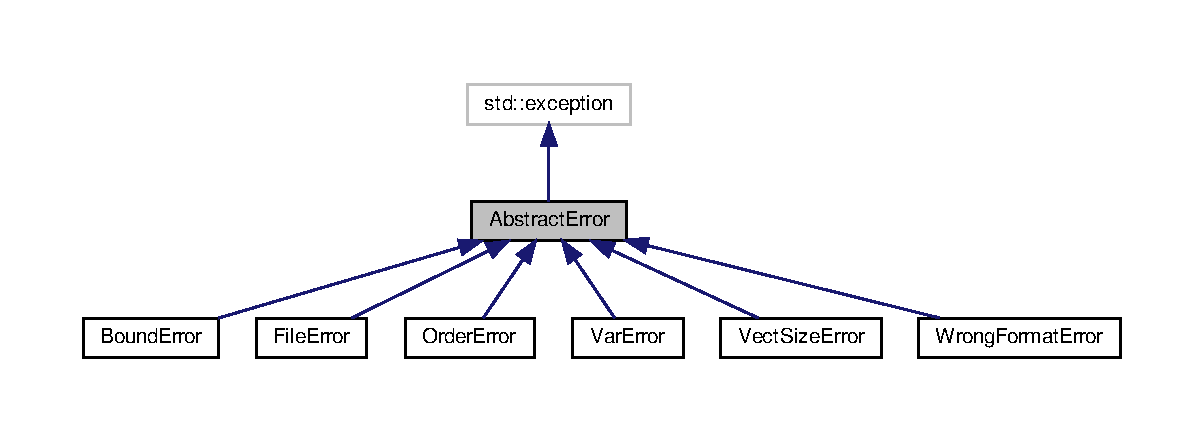
\includegraphics[width=350pt]{classAbstractError__inherit__graph}
\end{center}
\end{figure}


Collaboration diagram for Abstract\+Error\+:\nopagebreak
\begin{figure}[H]
\begin{center}
\leavevmode
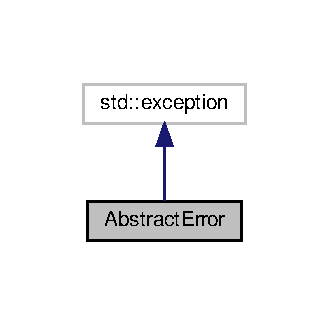
\includegraphics[width=158pt]{classAbstractError__coll__graph}
\end{center}
\end{figure}
\subsection*{Public Member Functions}
\begin{DoxyCompactItemize}
\item 
\hyperlink{classAbstractError_ae40c5440712bdcf91b2b7d733e2ee80b}{Abstract\+Error} ()
\item 
virtual \hyperlink{classAbstractError_a9b35711452ca3e32ac0609bcb493c181}{$\sim$\+Abstract\+Error} ()  throw ()
\item 
virtual const char $\ast$ \hyperlink{classAbstractError_a19735c7a9b5f6e84db606292967667a9}{what} () const  throw ()
\end{DoxyCompactItemize}


\subsection{Detailed Description}
Manages all errors encountered by the program. 

\subsection{Constructor \& Destructor Documentation}
\mbox{\Hypertarget{classAbstractError_ae40c5440712bdcf91b2b7d733e2ee80b}\label{classAbstractError_ae40c5440712bdcf91b2b7d733e2ee80b}} 
\index{Abstract\+Error@{Abstract\+Error}!Abstract\+Error@{Abstract\+Error}}
\index{Abstract\+Error@{Abstract\+Error}!Abstract\+Error@{Abstract\+Error}}
\subsubsection{\texorpdfstring{Abstract\+Error()}{AbstractError()}}
{\footnotesize\ttfamily Abstract\+Error\+::\+Abstract\+Error (\begin{DoxyParamCaption}{ }\end{DoxyParamCaption})\hspace{0.3cm}{\ttfamily [inline]}, {\ttfamily [explicit]}}

Constructor. \mbox{\Hypertarget{classAbstractError_a9b35711452ca3e32ac0609bcb493c181}\label{classAbstractError_a9b35711452ca3e32ac0609bcb493c181}} 
\index{Abstract\+Error@{Abstract\+Error}!````~Abstract\+Error@{$\sim$\+Abstract\+Error}}
\index{````~Abstract\+Error@{$\sim$\+Abstract\+Error}!Abstract\+Error@{Abstract\+Error}}
\subsubsection{\texorpdfstring{$\sim$\+Abstract\+Error()}{~AbstractError()}}
{\footnotesize\ttfamily virtual Abstract\+Error\+::$\sim$\+Abstract\+Error (\begin{DoxyParamCaption}{ }\end{DoxyParamCaption}) throw  ) \hspace{0.3cm}{\ttfamily [inline]}, {\ttfamily [virtual]}}

Destructor. Virtual to allow for subclassing. 

\subsection{Member Function Documentation}
\mbox{\Hypertarget{classAbstractError_a19735c7a9b5f6e84db606292967667a9}\label{classAbstractError_a19735c7a9b5f6e84db606292967667a9}} 
\index{Abstract\+Error@{Abstract\+Error}!what@{what}}
\index{what@{what}!Abstract\+Error@{Abstract\+Error}}
\subsubsection{\texorpdfstring{what()}{what()}}
{\footnotesize\ttfamily virtual const char$\ast$ Abstract\+Error\+::what (\begin{DoxyParamCaption}{ }\end{DoxyParamCaption}) const throw  ) \hspace{0.3cm}{\ttfamily [inline]}, {\ttfamily [virtual]}}

Returns a pointer to the (constant) error description. \begin{DoxyReturn}{Returns}
A pointer to a const char$\ast$. The underlying memory is in possession of the \hyperlink{classAbstractError}{Abstract\+Error} object. Callers must not attempt to free the memory. 
\end{DoxyReturn}


Reimplemented in \hyperlink{structWrongFormatError_a3c1c3f39ce135d19c7d0bb2fe8ddd3c1}{Wrong\+Format\+Error}, \hyperlink{structOrderError_a55140961b8a995ff9111a275cac708c8}{Order\+Error}, \hyperlink{structBoundError_a58ec01d9e329a9604cda74a8c273879a}{Bound\+Error}, \hyperlink{structVarError_a48ee904c5e61633cb6f4b9af2d093eaa}{Var\+Error}, \hyperlink{structVectSizeError_af92248320a9fb06b025662736a742c9e}{Vect\+Size\+Error}, and \hyperlink{structFileError_a7446417295daef00459e8d7e16cbb151}{File\+Error}.



The documentation for this class was generated from the following file\+:\begin{DoxyCompactItemize}
\item 
Modules/Abstract\+Error.\+h\end{DoxyCompactItemize}

\hypertarget{classAbstractExpectation}{}\section{Abstract\+Expectation Class Reference}
\label{classAbstractExpectation}\index{Abstract\+Expectation@{Abstract\+Expectation}}


Abstract class for expectations.  




{\ttfamily \#include $<$Abstract\+Expectation.\+h$>$}



Inheritance diagram for Abstract\+Expectation\+:\nopagebreak
\begin{figure}[H]
\begin{center}
\leavevmode
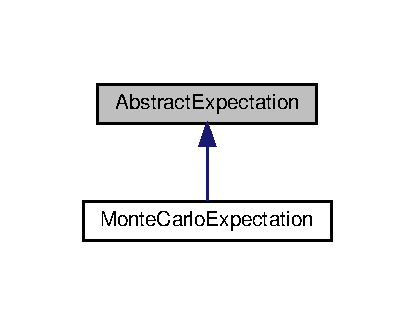
\includegraphics[width=199pt]{classAbstractExpectation__inherit__graph}
\end{center}
\end{figure}
\subsection*{Public Member Functions}
\begin{DoxyCompactItemize}
\item 
\mbox{\Hypertarget{classAbstractExpectation_ac2de8ff119a142ae9e6baf2bc28ee2a5}\label{classAbstractExpectation_ac2de8ff119a142ae9e6baf2bc28ee2a5}} 
\hyperlink{classAbstractExpectation_ac2de8ff119a142ae9e6baf2bc28ee2a5}{Abstract\+Expectation} ()
\begin{DoxyCompactList}\small\item\em Default Constructor. \end{DoxyCompactList}\item 
\mbox{\Hypertarget{classAbstractExpectation_af1eab325a354bc1444dd80fe572cf8a0}\label{classAbstractExpectation_af1eab325a354bc1444dd80fe572cf8a0}} 
virtual \hyperlink{classAbstractExpectation_af1eab325a354bc1444dd80fe572cf8a0}{$\sim$\+Abstract\+Expectation} ()
\begin{DoxyCompactList}\small\item\em Default Destructor. \end{DoxyCompactList}\item 
virtual double \hyperlink{classAbstractExpectation_a256d47c871d941e081a17194dda4d774}{get\+Expectation} () const =0
\begin{DoxyCompactList}\small\item\em Abstract function to get the computed expectation of the user defined function. \end{DoxyCompactList}\item 
virtual double \hyperlink{classAbstractExpectation_a3f3bc9fdcbd4856212857fc0fa4445a5}{evaluate\+Expectation} (const \hyperlink{classAbstractVariable}{Abstract\+Variable} $\ast$p\+Random)=0
\begin{DoxyCompactList}\small\item\em Abstract function to compute the expectation. \end{DoxyCompactList}\item 
virtual double \hyperlink{classAbstractExpectation_ac0fd8ea2ea546f6d01adec641886db14}{compute\+Mean} (const \hyperlink{classAbstractVariable}{Abstract\+Variable} $\ast$p\+Random)=0
\begin{DoxyCompactList}\small\item\em Abstract function to compute the mean of random samples. \end{DoxyCompactList}\end{DoxyCompactItemize}


\subsection{Detailed Description}
Abstract class for expectations. 

\subsection{Member Function Documentation}
\mbox{\Hypertarget{classAbstractExpectation_ac0fd8ea2ea546f6d01adec641886db14}\label{classAbstractExpectation_ac0fd8ea2ea546f6d01adec641886db14}} 
\index{Abstract\+Expectation@{Abstract\+Expectation}!compute\+Mean@{compute\+Mean}}
\index{compute\+Mean@{compute\+Mean}!Abstract\+Expectation@{Abstract\+Expectation}}
\subsubsection{\texorpdfstring{compute\+Mean()}{computeMean()}}
{\footnotesize\ttfamily virtual double Abstract\+Expectation\+::compute\+Mean (\begin{DoxyParamCaption}\item[{const \hyperlink{classAbstractVariable}{Abstract\+Variable} $\ast$}]{p\+Random }\end{DoxyParamCaption})\hspace{0.3cm}{\ttfamily [pure virtual]}}



Abstract function to compute the mean of random samples. 


\begin{DoxyParams}{Parameters}
{\em p\+Random} & \+: p\+Random \+: Pointer to a random variables. \\
\hline
\end{DoxyParams}
\begin{DoxyReturn}{Returns}
The mean of the random samples. 
\end{DoxyReturn}


Implemented in \hyperlink{classMonteCarloExpectation_a6f4489cc63ca48fcbf5f2cdd6258dfcc}{Monte\+Carlo\+Expectation}.

\mbox{\Hypertarget{classAbstractExpectation_a3f3bc9fdcbd4856212857fc0fa4445a5}\label{classAbstractExpectation_a3f3bc9fdcbd4856212857fc0fa4445a5}} 
\index{Abstract\+Expectation@{Abstract\+Expectation}!evaluate\+Expectation@{evaluate\+Expectation}}
\index{evaluate\+Expectation@{evaluate\+Expectation}!Abstract\+Expectation@{Abstract\+Expectation}}
\subsubsection{\texorpdfstring{evaluate\+Expectation()}{evaluateExpectation()}}
{\footnotesize\ttfamily virtual double Abstract\+Expectation\+::evaluate\+Expectation (\begin{DoxyParamCaption}\item[{const \hyperlink{classAbstractVariable}{Abstract\+Variable} $\ast$}]{p\+Random }\end{DoxyParamCaption})\hspace{0.3cm}{\ttfamily [pure virtual]}}



Abstract function to compute the expectation. 


\begin{DoxyParams}{Parameters}
{\em p\+Random} & \+: Pointer to a random variables. Used to evaluate the user function \\
\hline
\end{DoxyParams}
\begin{DoxyReturn}{Returns}
The expectation of the user defined function 
\end{DoxyReturn}


Implemented in \hyperlink{classMonteCarloExpectation_a3ded4ade26374189ab6d79f2c6928b0a}{Monte\+Carlo\+Expectation}.

\mbox{\Hypertarget{classAbstractExpectation_a256d47c871d941e081a17194dda4d774}\label{classAbstractExpectation_a256d47c871d941e081a17194dda4d774}} 
\index{Abstract\+Expectation@{Abstract\+Expectation}!get\+Expectation@{get\+Expectation}}
\index{get\+Expectation@{get\+Expectation}!Abstract\+Expectation@{Abstract\+Expectation}}
\subsubsection{\texorpdfstring{get\+Expectation()}{getExpectation()}}
{\footnotesize\ttfamily virtual double Abstract\+Expectation\+::get\+Expectation (\begin{DoxyParamCaption}{ }\end{DoxyParamCaption}) const\hspace{0.3cm}{\ttfamily [pure virtual]}}



Abstract function to get the computed expectation of the user defined function. 

\begin{DoxyReturn}{Returns}
The computed expectation 
\end{DoxyReturn}


Implemented in \hyperlink{classMonteCarloExpectation_a0cadc5362ae4d9073f4131ed9208053c}{Monte\+Carlo\+Expectation}.



The documentation for this class was generated from the following files\+:\begin{DoxyCompactItemize}
\item 
Modules/Abstract\+Expectation.\+h\item 
Modules/Abstract\+Expectation.\+cpp\end{DoxyCompactItemize}

\hypertarget{classAbstractFunc}{}\section{Abstract\+Func Class Reference}
\label{classAbstractFunc}\index{Abstract\+Func@{Abstract\+Func}}


Abstract class for functions.  




{\ttfamily \#include $<$Abstract\+Func.\+h$>$}



Inheritance diagram for Abstract\+Func\+:\nopagebreak
\begin{figure}[H]
\begin{center}
\leavevmode
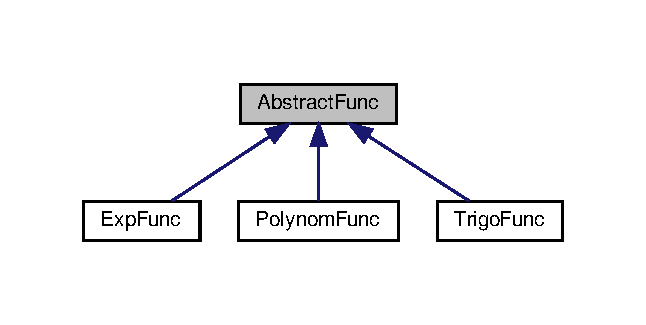
\includegraphics[width=310pt]{classAbstractFunc__inherit__graph}
\end{center}
\end{figure}
\subsection*{Public Member Functions}
\begin{DoxyCompactItemize}
\item 
\mbox{\Hypertarget{classAbstractFunc_a50a0d29bc7047f32e009a1bdaf481bc5}\label{classAbstractFunc_a50a0d29bc7047f32e009a1bdaf481bc5}} 
\hyperlink{classAbstractFunc_a50a0d29bc7047f32e009a1bdaf481bc5}{Abstract\+Func} ()
\begin{DoxyCompactList}\small\item\em Default Constructor. \end{DoxyCompactList}\item 
\hyperlink{classAbstractFunc_a2f8a88c02beff30adb2eb54346e8bb0f}{Abstract\+Func} (int a, int b)
\begin{DoxyCompactList}\small\item\em Constructor Construct a function with coefficient a and b (e.\+g \+: f(x) = ax+b) \end{DoxyCompactList}\item 
\mbox{\Hypertarget{classAbstractFunc_a9696320769335f8fea3e537b74032851}\label{classAbstractFunc_a9696320769335f8fea3e537b74032851}} 
virtual \hyperlink{classAbstractFunc_a9696320769335f8fea3e537b74032851}{$\sim$\+Abstract\+Func} ()
\begin{DoxyCompactList}\small\item\em Default Destructor. \end{DoxyCompactList}\item 
virtual double \hyperlink{classAbstractFunc_ac98be1daa5131b9fddcfdba0a2c34871}{evaluate} (double x)=0
\begin{DoxyCompactList}\small\item\em Abstract function to compute the evaluation of the user function on x \mbox{[}(f(x)\mbox{]}. \end{DoxyCompactList}\end{DoxyCompactItemize}
\subsection*{Protected Attributes}
\begin{DoxyCompactItemize}
\item 
\mbox{\Hypertarget{classAbstractFunc_ae4a1f381c5bc27564218bdc77b2c722e}\label{classAbstractFunc_ae4a1f381c5bc27564218bdc77b2c722e}} 
int {\bfseries coef\+\_\+a}
\item 
\mbox{\Hypertarget{classAbstractFunc_aefbfa8961c422c6f3c23adf0976061f2}\label{classAbstractFunc_aefbfa8961c422c6f3c23adf0976061f2}} 
int {\bfseries coef\+\_\+b}
\item 
\mbox{\Hypertarget{classAbstractFunc_afb8a73dd7c2c253de9fc88efc0ad99de}\label{classAbstractFunc_afb8a73dd7c2c253de9fc88efc0ad99de}} 
int {\bfseries order}
\end{DoxyCompactItemize}


\subsection{Detailed Description}
Abstract class for functions. 

\subsection{Constructor \& Destructor Documentation}
\mbox{\Hypertarget{classAbstractFunc_a2f8a88c02beff30adb2eb54346e8bb0f}\label{classAbstractFunc_a2f8a88c02beff30adb2eb54346e8bb0f}} 
\index{Abstract\+Func@{Abstract\+Func}!Abstract\+Func@{Abstract\+Func}}
\index{Abstract\+Func@{Abstract\+Func}!Abstract\+Func@{Abstract\+Func}}
\subsubsection{\texorpdfstring{Abstract\+Func()}{AbstractFunc()}}
{\footnotesize\ttfamily Abstract\+Func\+::\+Abstract\+Func (\begin{DoxyParamCaption}\item[{int}]{a,  }\item[{int}]{b }\end{DoxyParamCaption})\hspace{0.3cm}{\ttfamily [inline]}}



Constructor Construct a function with coefficient a and b (e.\+g \+: f(x) = ax+b) 


\begin{DoxyParams}{Parameters}
{\em a} & \+: First Coefficient \\
\hline
{\em b} & \+: Second CoefficientS \\
\hline
\end{DoxyParams}


\subsection{Member Function Documentation}
\mbox{\Hypertarget{classAbstractFunc_ac98be1daa5131b9fddcfdba0a2c34871}\label{classAbstractFunc_ac98be1daa5131b9fddcfdba0a2c34871}} 
\index{Abstract\+Func@{Abstract\+Func}!evaluate@{evaluate}}
\index{evaluate@{evaluate}!Abstract\+Func@{Abstract\+Func}}
\subsubsection{\texorpdfstring{evaluate()}{evaluate()}}
{\footnotesize\ttfamily virtual double Abstract\+Func\+::evaluate (\begin{DoxyParamCaption}\item[{double}]{x }\end{DoxyParamCaption})\hspace{0.3cm}{\ttfamily [pure virtual]}}



Abstract function to compute the evaluation of the user function on x \mbox{[}(f(x)\mbox{]}. 


\begin{DoxyParams}{Parameters}
{\em x} & \+: A random sample \\
\hline
\end{DoxyParams}
\begin{DoxyReturn}{Returns}
f(x) 
\end{DoxyReturn}


Implemented in \hyperlink{classPolynomFunc_a9908fc0cf0686123a98d3186d481fa6f}{Polynom\+Func}, \hyperlink{classTrigoFunc_ac04acbf2d2b7301d6e2084c9bb8daab2}{Trigo\+Func}, and \hyperlink{classExpFunc_a338e91308f12a66e3d1989ed5f589626}{Exp\+Func}.



The documentation for this class was generated from the following files\+:\begin{DoxyCompactItemize}
\item 
Modules/Abstract\+Func.\+h\item 
Modules/Abstract\+Func.\+cpp\end{DoxyCompactItemize}

\hypertarget{classAbstractReader}{}\section{Abstract\+Reader Class Reference}
\label{classAbstractReader}\index{Abstract\+Reader@{Abstract\+Reader}}


Abstract class for readers.  




{\ttfamily \#include $<$Abstract\+Reader.\+h$>$}



Inheritance diagram for Abstract\+Reader\+:\nopagebreak
\begin{figure}[H]
\begin{center}
\leavevmode
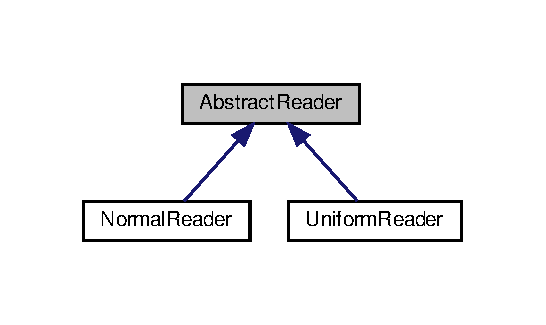
\includegraphics[width=262pt]{classAbstractReader__inherit__graph}
\end{center}
\end{figure}
\subsection*{Public Member Functions}
\begin{DoxyCompactItemize}
\item 
\mbox{\Hypertarget{classAbstractReader_afe9629707ae2c68bd9d10cc094dfcfc5}\label{classAbstractReader_afe9629707ae2c68bd9d10cc094dfcfc5}} 
\hyperlink{classAbstractReader_afe9629707ae2c68bd9d10cc094dfcfc5}{Abstract\+Reader} ()
\begin{DoxyCompactList}\small\item\em Default Constructor. \end{DoxyCompactList}\item 
\mbox{\Hypertarget{classAbstractReader_a18b9335ebe51ba66d0f449f95903f0dc}\label{classAbstractReader_a18b9335ebe51ba66d0f449f95903f0dc}} 
virtual \hyperlink{classAbstractReader_a18b9335ebe51ba66d0f449f95903f0dc}{$\sim$\+Abstract\+Reader} ()
\begin{DoxyCompactList}\small\item\em Default Destructor. \end{DoxyCompactList}\item 
virtual void \hyperlink{classAbstractReader_a01d009f3633d0af6d9ea8e34defda7f5}{read\+\_\+file} (const char $\ast$file\+\_\+name, \hyperlink{classAbstractVariable}{Abstract\+Variable} $\ast$\&p\+Random\+Variable)=0
\begin{DoxyCompactList}\small\item\em Abstract function to read the distribution file. \end{DoxyCompactList}\end{DoxyCompactItemize}


\subsection{Detailed Description}
Abstract class for readers. 

\subsection{Member Function Documentation}
\mbox{\Hypertarget{classAbstractReader_a01d009f3633d0af6d9ea8e34defda7f5}\label{classAbstractReader_a01d009f3633d0af6d9ea8e34defda7f5}} 
\index{Abstract\+Reader@{Abstract\+Reader}!read\+\_\+file@{read\+\_\+file}}
\index{read\+\_\+file@{read\+\_\+file}!Abstract\+Reader@{Abstract\+Reader}}
\subsubsection{\texorpdfstring{read\+\_\+file()}{read\_file()}}
{\footnotesize\ttfamily virtual void Abstract\+Reader\+::read\+\_\+file (\begin{DoxyParamCaption}\item[{const char $\ast$}]{file\+\_\+name,  }\item[{\hyperlink{classAbstractVariable}{Abstract\+Variable} $\ast$\&}]{p\+Random\+Variable }\end{DoxyParamCaption})\hspace{0.3cm}{\ttfamily [pure virtual]}}



Abstract function to read the distribution file. 


\begin{DoxyParams}{Parameters}
{\em file\+\_\+name} & \+: Distribution file name \\
\hline
{\em p\+Random\+Variable} & \+: Pointer to a Random variable \\
\hline
\end{DoxyParams}


Implemented in \hyperlink{classNormalReader_ae6571e3fdc414f143a5541807eded6e0}{Normal\+Reader}, and \hyperlink{classUniformReader_ae4e326a00cd72cdc1afa73beebe60ddc}{Uniform\+Reader}.



The documentation for this class was generated from the following files\+:\begin{DoxyCompactItemize}
\item 
Modules/Abstract\+Reader.\+h\item 
Modules/Abstract\+Reader.\+cpp\end{DoxyCompactItemize}

\hypertarget{classAbstractVariable}{}\section{Abstract\+Variable Class Reference}
\label{classAbstractVariable}\index{Abstract\+Variable@{Abstract\+Variable}}


Inheritance diagram for Abstract\+Variable\+:\nopagebreak
\begin{figure}[H]
\begin{center}
\leavevmode
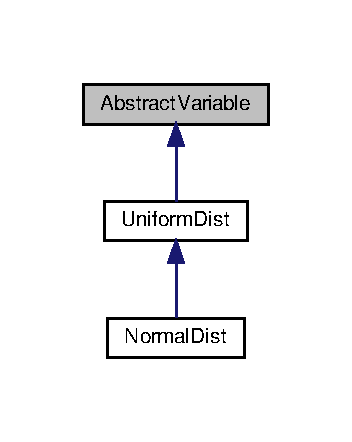
\includegraphics[width=169pt]{classAbstractVariable__inherit__graph}
\end{center}
\end{figure}
\subsection*{Public Member Functions}
\begin{DoxyCompactItemize}
\item 
virtual std\+::vector$<$ double $>$ \hyperlink{classAbstractVariable_a0312a988d8c527d2af7615ef2fd08621}{get\+\_\+vector} () const =0
\begin{DoxyCompactList}\small\item\em Abstract function to return the vector of generated random numbers. \end{DoxyCompactList}\item 
virtual double \hyperlink{classAbstractVariable_a99ceeeecc689a9683badfdfa7ef20c45}{get\+\_\+mean} () const =0
\begin{DoxyCompactList}\small\item\em Abstract function to return the mean of the distribution defined by the user. \end{DoxyCompactList}\item 
virtual double \hyperlink{classAbstractVariable_a71d378332b0e5b3c1760bb98db5d906b}{get\+\_\+var} () const =0
\begin{DoxyCompactList}\small\item\em Abstract function to return the variance of the distribution defined by the user. \end{DoxyCompactList}\item 
virtual int \hyperlink{classAbstractVariable_a96d9b63c3d9aff4673a9c66738302766}{get\+\_\+size} () const =0
\begin{DoxyCompactList}\small\item\em Abstract function to return the number of random numbers defined by the user. \end{DoxyCompactList}\end{DoxyCompactItemize}


\subsection{Member Function Documentation}
\mbox{\Hypertarget{classAbstractVariable_a99ceeeecc689a9683badfdfa7ef20c45}\label{classAbstractVariable_a99ceeeecc689a9683badfdfa7ef20c45}} 
\index{Abstract\+Variable@{Abstract\+Variable}!get\+\_\+mean@{get\+\_\+mean}}
\index{get\+\_\+mean@{get\+\_\+mean}!Abstract\+Variable@{Abstract\+Variable}}
\subsubsection{\texorpdfstring{get\+\_\+mean()}{get\_mean()}}
{\footnotesize\ttfamily virtual double Abstract\+Variable\+::get\+\_\+mean (\begin{DoxyParamCaption}{ }\end{DoxyParamCaption}) const\hspace{0.3cm}{\ttfamily [pure virtual]}}



Abstract function to return the mean of the distribution defined by the user. 

\begin{DoxyReturn}{Returns}
The mean of the distribution 
\end{DoxyReturn}


Implemented in \hyperlink{classNormalDist_a947707f47873251fd7857b4a7ed977bc}{Normal\+Dist}, and \hyperlink{classUniformDist_a18371ef0295e7aca4085015c0d844b41}{Uniform\+Dist}.

\mbox{\Hypertarget{classAbstractVariable_a96d9b63c3d9aff4673a9c66738302766}\label{classAbstractVariable_a96d9b63c3d9aff4673a9c66738302766}} 
\index{Abstract\+Variable@{Abstract\+Variable}!get\+\_\+size@{get\+\_\+size}}
\index{get\+\_\+size@{get\+\_\+size}!Abstract\+Variable@{Abstract\+Variable}}
\subsubsection{\texorpdfstring{get\+\_\+size()}{get\_size()}}
{\footnotesize\ttfamily virtual int Abstract\+Variable\+::get\+\_\+size (\begin{DoxyParamCaption}{ }\end{DoxyParamCaption}) const\hspace{0.3cm}{\ttfamily [pure virtual]}}



Abstract function to return the number of random numbers defined by the user. 

\begin{DoxyReturn}{Returns}
The number of random numbers 
\end{DoxyReturn}


Implemented in \hyperlink{classNormalDist_a6dcfba2a8149dbd527392c32b3d7a7a1}{Normal\+Dist}, and \hyperlink{classUniformDist_a6e7a871053b2eb563fcbf2f7e02fb22b}{Uniform\+Dist}.

\mbox{\Hypertarget{classAbstractVariable_a71d378332b0e5b3c1760bb98db5d906b}\label{classAbstractVariable_a71d378332b0e5b3c1760bb98db5d906b}} 
\index{Abstract\+Variable@{Abstract\+Variable}!get\+\_\+var@{get\+\_\+var}}
\index{get\+\_\+var@{get\+\_\+var}!Abstract\+Variable@{Abstract\+Variable}}
\subsubsection{\texorpdfstring{get\+\_\+var()}{get\_var()}}
{\footnotesize\ttfamily virtual double Abstract\+Variable\+::get\+\_\+var (\begin{DoxyParamCaption}{ }\end{DoxyParamCaption}) const\hspace{0.3cm}{\ttfamily [pure virtual]}}



Abstract function to return the variance of the distribution defined by the user. 

\begin{DoxyReturn}{Returns}
The variance of the distribution 
\end{DoxyReturn}


Implemented in \hyperlink{classNormalDist_a46bc646f126ac3c2d46bcd9ccbf01135}{Normal\+Dist}, and \hyperlink{classUniformDist_aade143a6ff9ed9a8bee2e6b9fb2fed4c}{Uniform\+Dist}.

\mbox{\Hypertarget{classAbstractVariable_a0312a988d8c527d2af7615ef2fd08621}\label{classAbstractVariable_a0312a988d8c527d2af7615ef2fd08621}} 
\index{Abstract\+Variable@{Abstract\+Variable}!get\+\_\+vector@{get\+\_\+vector}}
\index{get\+\_\+vector@{get\+\_\+vector}!Abstract\+Variable@{Abstract\+Variable}}
\subsubsection{\texorpdfstring{get\+\_\+vector()}{get\_vector()}}
{\footnotesize\ttfamily virtual std\+::vector$<$double$>$ Abstract\+Variable\+::get\+\_\+vector (\begin{DoxyParamCaption}{ }\end{DoxyParamCaption}) const\hspace{0.3cm}{\ttfamily [pure virtual]}}



Abstract function to return the vector of generated random numbers. 

\begin{DoxyReturn}{Returns}
A vector of generated random numbers 
\end{DoxyReturn}


Implemented in \hyperlink{classNormalDist_a473e67b9d1787f6ff887f6854dbd350c}{Normal\+Dist}, and \hyperlink{classUniformDist_a60df487bfb003628e9997ebcb5aedcde}{Uniform\+Dist}.



The documentation for this class was generated from the following file\+:\begin{DoxyCompactItemize}
\item 
Modules/Abstract\+Variable.\+h\end{DoxyCompactItemize}

\hypertarget{structBoundError}{}\section{Bound\+Error Struct Reference}
\label{structBoundError}\index{Bound\+Error@{Bound\+Error}}


Inheritance diagram for Bound\+Error\+:\nopagebreak
\begin{figure}[H]
\begin{center}
\leavevmode
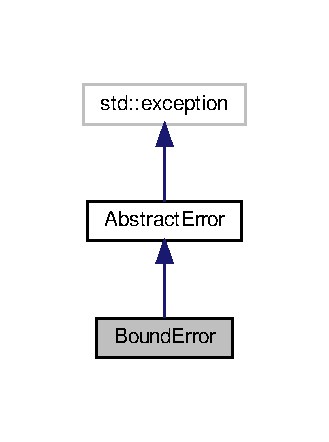
\includegraphics[width=158pt]{structBoundError__inherit__graph}
\end{center}
\end{figure}


Collaboration diagram for Bound\+Error\+:\nopagebreak
\begin{figure}[H]
\begin{center}
\leavevmode
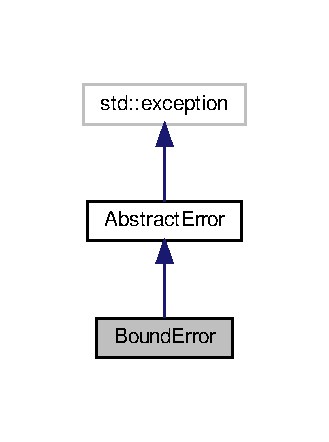
\includegraphics[width=158pt]{structBoundError__coll__graph}
\end{center}
\end{figure}
\subsection*{Public Member Functions}
\begin{DoxyCompactItemize}
\item 
const char $\ast$ \hyperlink{structBoundError_a58ec01d9e329a9604cda74a8c273879a}{what} () const override  throw ()
\end{DoxyCompactItemize}


\subsection{Member Function Documentation}
\mbox{\Hypertarget{structBoundError_a58ec01d9e329a9604cda74a8c273879a}\label{structBoundError_a58ec01d9e329a9604cda74a8c273879a}} 
\index{Bound\+Error@{Bound\+Error}!what@{what}}
\index{what@{what}!Bound\+Error@{Bound\+Error}}
\subsubsection{\texorpdfstring{what()}{what()}}
{\footnotesize\ttfamily const char$\ast$ Bound\+Error\+::what (\begin{DoxyParamCaption}{ }\end{DoxyParamCaption}) const throw  ) \hspace{0.3cm}{\ttfamily [inline]}, {\ttfamily [override]}, {\ttfamily [virtual]}}

Returns a pointer to the (constant) error description. \begin{DoxyReturn}{Returns}
A pointer to a const char$\ast$. The underlying memory is in possession of the \hyperlink{classAbstractError}{Abstract\+Error} object. Callers must not attempt to free the memory. 
\end{DoxyReturn}


Reimplemented from \hyperlink{classAbstractError_a19735c7a9b5f6e84db606292967667a9}{Abstract\+Error}.



The documentation for this struct was generated from the following file\+:\begin{DoxyCompactItemize}
\item 
Modules/Abstract\+Error.\+h\end{DoxyCompactItemize}

\hypertarget{classCentralLimitThm}{}\section{Central\+Limit\+Thm Class Reference}
\label{classCentralLimitThm}\index{Central\+Limit\+Thm@{Central\+Limit\+Thm}}


Class to verify the C\+TL theorem.  




{\ttfamily \#include $<$Central\+Limit\+Thm.\+h$>$}

\subsection*{Public Member Functions}
\begin{DoxyCompactItemize}
\item 
\mbox{\Hypertarget{classCentralLimitThm_a70d886fa3a13dd2e3dbe7bc6c996fb2f}\label{classCentralLimitThm_a70d886fa3a13dd2e3dbe7bc6c996fb2f}} 
\hyperlink{classCentralLimitThm_a70d886fa3a13dd2e3dbe7bc6c996fb2f}{Central\+Limit\+Thm} ()
\begin{DoxyCompactList}\small\item\em Default Constructor. \end{DoxyCompactList}\item 
\mbox{\Hypertarget{classCentralLimitThm_acd4def2fc5647a486a5c766a7f8a61b2}\label{classCentralLimitThm_acd4def2fc5647a486a5c766a7f8a61b2}} 
\hyperlink{classCentralLimitThm_acd4def2fc5647a486a5c766a7f8a61b2}{$\sim$\+Central\+Limit\+Thm} ()
\begin{DoxyCompactList}\small\item\em Default Destructor. \end{DoxyCompactList}\item 
\hyperlink{classCentralLimitThm_a41cc29d0165ac8738d926593a43fd586}{Central\+Limit\+Thm} (\hyperlink{classAbstractVariable}{Abstract\+Variable} $\ast$p\+Random, int multiples)
\begin{DoxyCompactList}\small\item\em Constructor Define a new csv file to save the means of generated samples of same size. \end{DoxyCompactList}\item 
void \hyperlink{classCentralLimitThm_a3898fbea7b16e86a2632914abbe67704}{verify\+\_\+thm} (\hyperlink{classAbstractVariable}{Abstract\+Variable} $\ast$p\+Random, \hyperlink{classAbstractExpectation}{Abstract\+Expectation} $\ast$p\+Expectation)
\begin{DoxyCompactList}\small\item\em Compute the mean of the random samples and append it to the existing csv file. \end{DoxyCompactList}\end{DoxyCompactItemize}


\subsection{Detailed Description}
Class to verify the C\+TL theorem. 

\subsection{Constructor \& Destructor Documentation}
\mbox{\Hypertarget{classCentralLimitThm_a41cc29d0165ac8738d926593a43fd586}\label{classCentralLimitThm_a41cc29d0165ac8738d926593a43fd586}} 
\index{Central\+Limit\+Thm@{Central\+Limit\+Thm}!Central\+Limit\+Thm@{Central\+Limit\+Thm}}
\index{Central\+Limit\+Thm@{Central\+Limit\+Thm}!Central\+Limit\+Thm@{Central\+Limit\+Thm}}
\subsubsection{\texorpdfstring{Central\+Limit\+Thm()}{CentralLimitThm()}}
{\footnotesize\ttfamily Central\+Limit\+Thm\+::\+Central\+Limit\+Thm (\begin{DoxyParamCaption}\item[{\hyperlink{classAbstractVariable}{Abstract\+Variable} $\ast$}]{p\+Random,  }\item[{int}]{multiples }\end{DoxyParamCaption})}



Constructor Define a new csv file to save the means of generated samples of same size. 


\begin{DoxyParams}{Parameters}
{\em p\+Random} & \+: Pointer of initially generated random samples \\
\hline
{\em multiples} & \+: define the size of the new samples (N,2N,3N ...) \\
\hline
\end{DoxyParams}


\subsection{Member Function Documentation}
\mbox{\Hypertarget{classCentralLimitThm_a3898fbea7b16e86a2632914abbe67704}\label{classCentralLimitThm_a3898fbea7b16e86a2632914abbe67704}} 
\index{Central\+Limit\+Thm@{Central\+Limit\+Thm}!verify\+\_\+thm@{verify\+\_\+thm}}
\index{verify\+\_\+thm@{verify\+\_\+thm}!Central\+Limit\+Thm@{Central\+Limit\+Thm}}
\subsubsection{\texorpdfstring{verify\+\_\+thm()}{verify\_thm()}}
{\footnotesize\ttfamily void Central\+Limit\+Thm\+::verify\+\_\+thm (\begin{DoxyParamCaption}\item[{\hyperlink{classAbstractVariable}{Abstract\+Variable} $\ast$}]{p\+Random,  }\item[{\hyperlink{classAbstractExpectation}{Abstract\+Expectation} $\ast$}]{p\+Expectation }\end{DoxyParamCaption})}



Compute the mean of the random samples and append it to the existing csv file. 


\begin{DoxyParams}{Parameters}
{\em p\+Random} & \+: Pointer of generated random samples \\
\hline
{\em p\+Expectation} & \+: Pointer of Monte\+Carlo Expectation \\
\hline
\end{DoxyParams}


The documentation for this class was generated from the following files\+:\begin{DoxyCompactItemize}
\item 
Modules/Central\+Limit\+Thm.\+h\item 
Modules/Central\+Limit\+Thm.\+cpp\end{DoxyCompactItemize}

\hypertarget{classExpFunc}{}\section{Exp\+Func Class Reference}
\label{classExpFunc}\index{Exp\+Func@{Exp\+Func}}


Exponential function class Derived from \hyperlink{classAbstractFunc}{Abstract\+Func}.  




{\ttfamily \#include $<$Exp\+Func.\+h$>$}



Inheritance diagram for Exp\+Func\+:\nopagebreak
\begin{figure}[H]
\begin{center}
\leavevmode
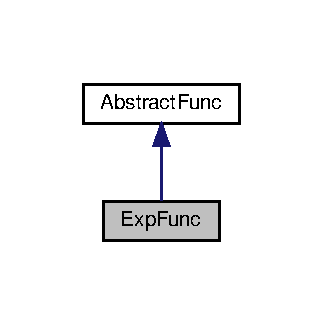
\includegraphics[width=155pt]{classExpFunc__inherit__graph}
\end{center}
\end{figure}


Collaboration diagram for Exp\+Func\+:\nopagebreak
\begin{figure}[H]
\begin{center}
\leavevmode
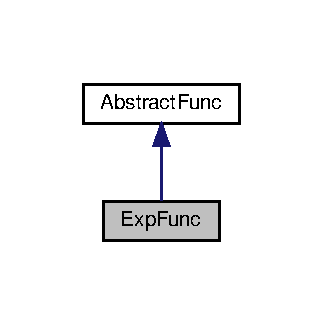
\includegraphics[width=155pt]{classExpFunc__coll__graph}
\end{center}
\end{figure}
\subsection*{Public Member Functions}
\begin{DoxyCompactItemize}
\item 
\mbox{\Hypertarget{classExpFunc_a92994226f51d2c3d360df145e3720721}\label{classExpFunc_a92994226f51d2c3d360df145e3720721}} 
\hyperlink{classExpFunc_a92994226f51d2c3d360df145e3720721}{Exp\+Func} ()
\begin{DoxyCompactList}\small\item\em Default Constructor. \end{DoxyCompactList}\item 
\mbox{\Hypertarget{classExpFunc_acfad0935316f9182e83f39949fc63c2c}\label{classExpFunc_acfad0935316f9182e83f39949fc63c2c}} 
\hyperlink{classExpFunc_acfad0935316f9182e83f39949fc63c2c}{$\sim$\+Exp\+Func} ()
\begin{DoxyCompactList}\small\item\em Default Destructor. \end{DoxyCompactList}\item 
\hyperlink{classExpFunc_a3dde289a9b9da2d3d830f71f15b4a762}{Exp\+Func} (int a, int b)
\begin{DoxyCompactList}\small\item\em Constructor Define the function \char`\"{}be$\ast$xp(ax)\char`\"{}. \end{DoxyCompactList}\item 
double \hyperlink{classExpFunc_a338e91308f12a66e3d1989ed5f589626}{evaluate} (double x)
\begin{DoxyCompactList}\small\item\em Return the evaluation of the user exponential function on a random number. \end{DoxyCompactList}\end{DoxyCompactItemize}
\subsection*{Additional Inherited Members}


\subsection{Detailed Description}
Exponential function class Derived from \hyperlink{classAbstractFunc}{Abstract\+Func}. 

\subsection{Constructor \& Destructor Documentation}
\mbox{\Hypertarget{classExpFunc_a3dde289a9b9da2d3d830f71f15b4a762}\label{classExpFunc_a3dde289a9b9da2d3d830f71f15b4a762}} 
\index{Exp\+Func@{Exp\+Func}!Exp\+Func@{Exp\+Func}}
\index{Exp\+Func@{Exp\+Func}!Exp\+Func@{Exp\+Func}}
\subsubsection{\texorpdfstring{Exp\+Func()}{ExpFunc()}}
{\footnotesize\ttfamily Exp\+Func\+::\+Exp\+Func (\begin{DoxyParamCaption}\item[{int}]{a,  }\item[{int}]{b }\end{DoxyParamCaption})\hspace{0.3cm}{\ttfamily [inline]}}



Constructor Define the function \char`\"{}be$\ast$xp(ax)\char`\"{}. 


\begin{DoxyParams}{Parameters}
{\em a} & \+: Second Coefficient \\
\hline
{\em b} & \+: First Coefficient \\
\hline
\end{DoxyParams}


\subsection{Member Function Documentation}
\mbox{\Hypertarget{classExpFunc_a338e91308f12a66e3d1989ed5f589626}\label{classExpFunc_a338e91308f12a66e3d1989ed5f589626}} 
\index{Exp\+Func@{Exp\+Func}!evaluate@{evaluate}}
\index{evaluate@{evaluate}!Exp\+Func@{Exp\+Func}}
\subsubsection{\texorpdfstring{evaluate()}{evaluate()}}
{\footnotesize\ttfamily double Exp\+Func\+::evaluate (\begin{DoxyParamCaption}\item[{double}]{x }\end{DoxyParamCaption})\hspace{0.3cm}{\ttfamily [virtual]}}



Return the evaluation of the user exponential function on a random number. 


\begin{DoxyParams}{Parameters}
{\em x} & \+: a Random number \\
\hline
\end{DoxyParams}
\begin{DoxyReturn}{Returns}
\+: b$\ast$exp(ax) 
\end{DoxyReturn}


Implements \hyperlink{classAbstractFunc_ac98be1daa5131b9fddcfdba0a2c34871}{Abstract\+Func}.



The documentation for this class was generated from the following files\+:\begin{DoxyCompactItemize}
\item 
Modules/Exp\+Func.\+h\item 
Modules/Exp\+Func.\+cpp\end{DoxyCompactItemize}

\hypertarget{structFileError}{}\section{File\+Error Struct Reference}
\label{structFileError}\index{File\+Error@{File\+Error}}


Inheritance diagram for File\+Error\+:\nopagebreak
\begin{figure}[H]
\begin{center}
\leavevmode
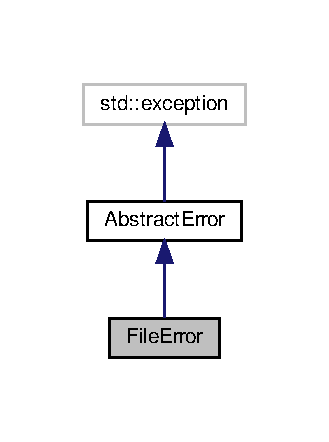
\includegraphics[width=158pt]{structFileError__inherit__graph}
\end{center}
\end{figure}


Collaboration diagram for File\+Error\+:\nopagebreak
\begin{figure}[H]
\begin{center}
\leavevmode
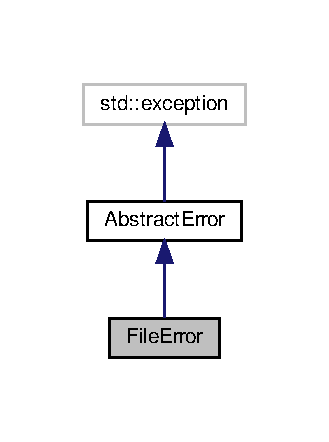
\includegraphics[width=158pt]{structFileError__coll__graph}
\end{center}
\end{figure}
\subsection*{Public Member Functions}
\begin{DoxyCompactItemize}
\item 
const char $\ast$ \hyperlink{structFileError_a7446417295daef00459e8d7e16cbb151}{what} () const override  throw ()
\end{DoxyCompactItemize}


\subsection{Member Function Documentation}
\mbox{\Hypertarget{structFileError_a7446417295daef00459e8d7e16cbb151}\label{structFileError_a7446417295daef00459e8d7e16cbb151}} 
\index{File\+Error@{File\+Error}!what@{what}}
\index{what@{what}!File\+Error@{File\+Error}}
\subsubsection{\texorpdfstring{what()}{what()}}
{\footnotesize\ttfamily const char$\ast$ File\+Error\+::what (\begin{DoxyParamCaption}{ }\end{DoxyParamCaption}) const throw  ) \hspace{0.3cm}{\ttfamily [inline]}, {\ttfamily [override]}, {\ttfamily [virtual]}}

Returns a pointer to the (constant) error description. \begin{DoxyReturn}{Returns}
A pointer to a const char$\ast$. The underlying memory is in possession of the \hyperlink{classAbstractError}{Abstract\+Error} object. Callers must not attempt to free the memory. 
\end{DoxyReturn}


Reimplemented from \hyperlink{classAbstractError_a19735c7a9b5f6e84db606292967667a9}{Abstract\+Error}.



The documentation for this struct was generated from the following file\+:\begin{DoxyCompactItemize}
\item 
Modules/Abstract\+Error.\+h\end{DoxyCompactItemize}

\hypertarget{classFunctReader}{}\section{Funct\+Reader Class Reference}
\label{classFunctReader}\index{Funct\+Reader@{Funct\+Reader}}


Function reader class.  




{\ttfamily \#include $<$Funct\+Reader.\+h$>$}

\subsection*{Public Member Functions}
\begin{DoxyCompactItemize}
\item 
\mbox{\Hypertarget{classFunctReader_ab128a05e403d3ed94f0bd558438b9bf0}\label{classFunctReader_ab128a05e403d3ed94f0bd558438b9bf0}} 
\hyperlink{classFunctReader_ab128a05e403d3ed94f0bd558438b9bf0}{Funct\+Reader} ()
\begin{DoxyCompactList}\small\item\em Default Constructor. \end{DoxyCompactList}\item 
\mbox{\Hypertarget{classFunctReader_ac1c092a6a2536afeef2fcc187eb240aa}\label{classFunctReader_ac1c092a6a2536afeef2fcc187eb240aa}} 
\hyperlink{classFunctReader_ac1c092a6a2536afeef2fcc187eb240aa}{$\sim$\+Funct\+Reader} ()
\begin{DoxyCompactList}\small\item\em Default Destructor. \end{DoxyCompactList}\item 
void \hyperlink{classFunctReader_a6951ceadd525807718b17d951c916fae}{read\+\_\+file} (const char $\ast$file, \hyperlink{classAbstractFunc}{Abstract\+Func} $\ast$\&p\+Function, int \&order)
\begin{DoxyCompactList}\small\item\em Read file for user function type and coefficients. \end{DoxyCompactList}\end{DoxyCompactItemize}


\subsection{Detailed Description}
Function reader class. 

\subsection{Member Function Documentation}
\mbox{\Hypertarget{classFunctReader_a6951ceadd525807718b17d951c916fae}\label{classFunctReader_a6951ceadd525807718b17d951c916fae}} 
\index{Funct\+Reader@{Funct\+Reader}!read\+\_\+file@{read\+\_\+file}}
\index{read\+\_\+file@{read\+\_\+file}!Funct\+Reader@{Funct\+Reader}}
\subsubsection{\texorpdfstring{read\+\_\+file()}{read\_file()}}
{\footnotesize\ttfamily void Funct\+Reader\+::read\+\_\+file (\begin{DoxyParamCaption}\item[{const char $\ast$}]{file,  }\item[{\hyperlink{classAbstractFunc}{Abstract\+Func} $\ast$\&}]{p\+Function,  }\item[{int \&}]{order }\end{DoxyParamCaption})}



Read file for user function type and coefficients. 


\begin{DoxyParams}{Parameters}
{\em file} & \+: file name \\
\hline
{\em p\+Function} & \+: Pointer to a user function \\
\hline
{\em order} & \+: Order defined by the user \\
\hline
\end{DoxyParams}


The documentation for this class was generated from the following files\+:\begin{DoxyCompactItemize}
\item 
Modules/Funct\+Reader.\+h\item 
Modules/Funct\+Reader.\+cpp\end{DoxyCompactItemize}

\hypertarget{classMonteCarloExpectation}{}\section{Monte\+Carlo\+Expectation Class Reference}
\label{classMonteCarloExpectation}\index{Monte\+Carlo\+Expectation@{Monte\+Carlo\+Expectation}}


Class to compute the monte carlo expectation of a sample Derived form \hyperlink{classAbstractExpectation}{Abstract\+Expectation} class.  




{\ttfamily \#include $<$Monte\+Carlo\+Expectation.\+h$>$}



Inheritance diagram for Monte\+Carlo\+Expectation\+:\nopagebreak
\begin{figure}[H]
\begin{center}
\leavevmode
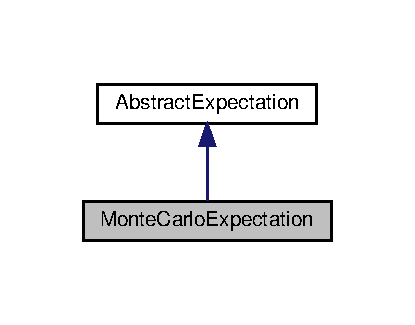
\includegraphics[width=199pt]{classMonteCarloExpectation__inherit__graph}
\end{center}
\end{figure}


Collaboration diagram for Monte\+Carlo\+Expectation\+:\nopagebreak
\begin{figure}[H]
\begin{center}
\leavevmode
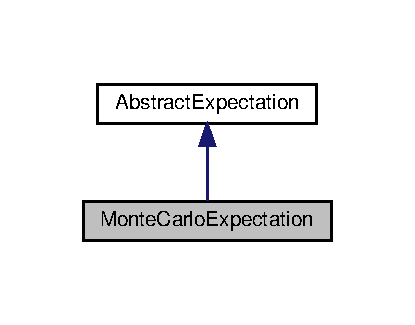
\includegraphics[width=199pt]{classMonteCarloExpectation__coll__graph}
\end{center}
\end{figure}
\subsection*{Public Member Functions}
\begin{DoxyCompactItemize}
\item 
\mbox{\Hypertarget{classMonteCarloExpectation_a503c5564902dd9b808181de315b93f5c}\label{classMonteCarloExpectation_a503c5564902dd9b808181de315b93f5c}} 
\hyperlink{classMonteCarloExpectation_a503c5564902dd9b808181de315b93f5c}{Monte\+Carlo\+Expectation} ()
\begin{DoxyCompactList}\small\item\em Default constructor. \end{DoxyCompactList}\item 
\mbox{\Hypertarget{classMonteCarloExpectation_a584a93ef10f6e75ca60939c3ed0b1468}\label{classMonteCarloExpectation_a584a93ef10f6e75ca60939c3ed0b1468}} 
\hyperlink{classMonteCarloExpectation_a584a93ef10f6e75ca60939c3ed0b1468}{$\sim$\+Monte\+Carlo\+Expectation} ()
\begin{DoxyCompactList}\small\item\em Default Destructor. \end{DoxyCompactList}\item 
\hyperlink{classMonteCarloExpectation_ad595bc1f4a61d0138fd1d55e11b4d267}{Monte\+Carlo\+Expectation} (\hyperlink{classAbstractFunc}{Abstract\+Func} $\ast$p\+Function, const \hyperlink{classAbstractVariable}{Abstract\+Variable} $\ast$p\+Random)
\begin{DoxyCompactList}\small\item\em Constructor Defines the user\textquotesingle{}s function and the expectation. \end{DoxyCompactList}\item 
double \hyperlink{classMonteCarloExpectation_a0cadc5362ae4d9073f4131ed9208053c}{get\+Expectation} () const
\begin{DoxyCompactList}\small\item\em Returns the value of the previously computed expectation. \end{DoxyCompactList}\item 
double \hyperlink{classMonteCarloExpectation_a3ded4ade26374189ab6d79f2c6928b0a}{evaluate\+Expectation} (const \hyperlink{classAbstractVariable}{Abstract\+Variable} $\ast$p\+Random)
\begin{DoxyCompactList}\small\item\em Computes the value of the expctetation for a given function depending on the distribution of p\+Random. \end{DoxyCompactList}\item 
double \hyperlink{classMonteCarloExpectation_a6f4489cc63ca48fcbf5f2cdd6258dfcc}{compute\+Mean} (const \hyperlink{classAbstractVariable}{Abstract\+Variable} $\ast$p\+Random)
\begin{DoxyCompactList}\small\item\em Computes the mean of a given distribution. \end{DoxyCompactList}\end{DoxyCompactItemize}


\subsection{Detailed Description}
Class to compute the monte carlo expectation of a sample Derived form \hyperlink{classAbstractExpectation}{Abstract\+Expectation} class. 

\subsection{Constructor \& Destructor Documentation}
\mbox{\Hypertarget{classMonteCarloExpectation_ad595bc1f4a61d0138fd1d55e11b4d267}\label{classMonteCarloExpectation_ad595bc1f4a61d0138fd1d55e11b4d267}} 
\index{Monte\+Carlo\+Expectation@{Monte\+Carlo\+Expectation}!Monte\+Carlo\+Expectation@{Monte\+Carlo\+Expectation}}
\index{Monte\+Carlo\+Expectation@{Monte\+Carlo\+Expectation}!Monte\+Carlo\+Expectation@{Monte\+Carlo\+Expectation}}
\subsubsection{\texorpdfstring{Monte\+Carlo\+Expectation()}{MonteCarloExpectation()}}
{\footnotesize\ttfamily Monte\+Carlo\+Expectation\+::\+Monte\+Carlo\+Expectation (\begin{DoxyParamCaption}\item[{\hyperlink{classAbstractFunc}{Abstract\+Func} $\ast$}]{p\+Function,  }\item[{const \hyperlink{classAbstractVariable}{Abstract\+Variable} $\ast$}]{p\+Random }\end{DoxyParamCaption})}



Constructor Defines the user\textquotesingle{}s function and the expectation. 


\begin{DoxyParams}{Parameters}
{\em p\+Function} & Pointer to the user defined function. \\
\hline
{\em p\+Random} & Pointer to the previously defined distibution. \\
\hline
\end{DoxyParams}


\subsection{Member Function Documentation}
\mbox{\Hypertarget{classMonteCarloExpectation_a6f4489cc63ca48fcbf5f2cdd6258dfcc}\label{classMonteCarloExpectation_a6f4489cc63ca48fcbf5f2cdd6258dfcc}} 
\index{Monte\+Carlo\+Expectation@{Monte\+Carlo\+Expectation}!compute\+Mean@{compute\+Mean}}
\index{compute\+Mean@{compute\+Mean}!Monte\+Carlo\+Expectation@{Monte\+Carlo\+Expectation}}
\subsubsection{\texorpdfstring{compute\+Mean()}{computeMean()}}
{\footnotesize\ttfamily double Monte\+Carlo\+Expectation\+::compute\+Mean (\begin{DoxyParamCaption}\item[{const \hyperlink{classAbstractVariable}{Abstract\+Variable} $\ast$}]{p\+Random }\end{DoxyParamCaption})\hspace{0.3cm}{\ttfamily [virtual]}}



Computes the mean of a given distribution. 


\begin{DoxyParams}{Parameters}
{\em p\+Random} & Pointer to the previously defined distibution. \\
\hline
\end{DoxyParams}
\begin{DoxyReturn}{Returns}
The value of the mean. 
\end{DoxyReturn}


Implements \hyperlink{classAbstractExpectation_ac0fd8ea2ea546f6d01adec641886db14}{Abstract\+Expectation}.

\mbox{\Hypertarget{classMonteCarloExpectation_a3ded4ade26374189ab6d79f2c6928b0a}\label{classMonteCarloExpectation_a3ded4ade26374189ab6d79f2c6928b0a}} 
\index{Monte\+Carlo\+Expectation@{Monte\+Carlo\+Expectation}!evaluate\+Expectation@{evaluate\+Expectation}}
\index{evaluate\+Expectation@{evaluate\+Expectation}!Monte\+Carlo\+Expectation@{Monte\+Carlo\+Expectation}}
\subsubsection{\texorpdfstring{evaluate\+Expectation()}{evaluateExpectation()}}
{\footnotesize\ttfamily double Monte\+Carlo\+Expectation\+::evaluate\+Expectation (\begin{DoxyParamCaption}\item[{const \hyperlink{classAbstractVariable}{Abstract\+Variable} $\ast$}]{p\+Random }\end{DoxyParamCaption})\hspace{0.3cm}{\ttfamily [virtual]}}



Computes the value of the expctetation for a given function depending on the distribution of p\+Random. 


\begin{DoxyParams}{Parameters}
{\em p\+Random} & Pointer to the previously defined distibution. \\
\hline
\end{DoxyParams}
\begin{DoxyReturn}{Returns}
The value of the expectation. 
\end{DoxyReturn}


Implements \hyperlink{classAbstractExpectation_a3f3bc9fdcbd4856212857fc0fa4445a5}{Abstract\+Expectation}.

\mbox{\Hypertarget{classMonteCarloExpectation_a0cadc5362ae4d9073f4131ed9208053c}\label{classMonteCarloExpectation_a0cadc5362ae4d9073f4131ed9208053c}} 
\index{Monte\+Carlo\+Expectation@{Monte\+Carlo\+Expectation}!get\+Expectation@{get\+Expectation}}
\index{get\+Expectation@{get\+Expectation}!Monte\+Carlo\+Expectation@{Monte\+Carlo\+Expectation}}
\subsubsection{\texorpdfstring{get\+Expectation()}{getExpectation()}}
{\footnotesize\ttfamily double Monte\+Carlo\+Expectation\+::get\+Expectation (\begin{DoxyParamCaption}{ }\end{DoxyParamCaption}) const\hspace{0.3cm}{\ttfamily [inline]}, {\ttfamily [virtual]}}



Returns the value of the previously computed expectation. 

\begin{DoxyReturn}{Returns}
The value of the expectation. 
\end{DoxyReturn}


Implements \hyperlink{classAbstractExpectation_a256d47c871d941e081a17194dda4d774}{Abstract\+Expectation}.



The documentation for this class was generated from the following files\+:\begin{DoxyCompactItemize}
\item 
Modules/Monte\+Carlo\+Expectation.\+h\item 
Modules/Monte\+Carlo\+Expectation.\+cpp\end{DoxyCompactItemize}

\hypertarget{classNormalDist}{}\section{Normal\+Dist Class Reference}
\label{classNormalDist}\index{Normal\+Dist@{Normal\+Dist}}


Class to create a normal distribution sample using inverse transform sampling Derived from \hyperlink{classUniformDist}{Uniform\+Dist} since the inverse transform sampling is based on uniform distributed sample between 0 and 1.  




{\ttfamily \#include $<$Normal\+Dist.\+h$>$}



Inheritance diagram for Normal\+Dist\+:\nopagebreak
\begin{figure}[H]
\begin{center}
\leavevmode
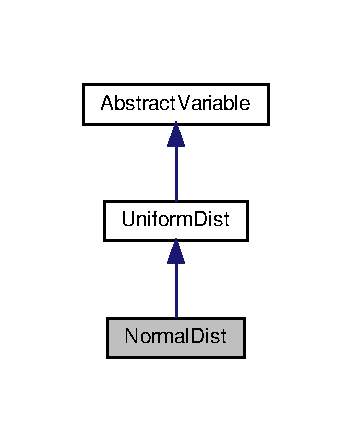
\includegraphics[width=169pt]{classNormalDist__inherit__graph}
\end{center}
\end{figure}


Collaboration diagram for Normal\+Dist\+:\nopagebreak
\begin{figure}[H]
\begin{center}
\leavevmode
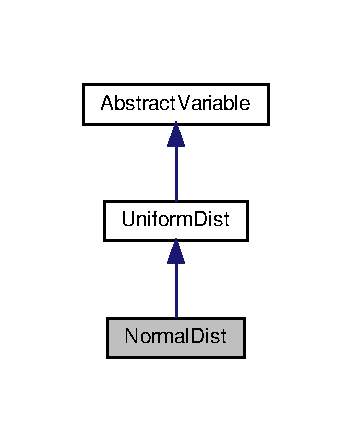
\includegraphics[width=169pt]{classNormalDist__coll__graph}
\end{center}
\end{figure}
\subsection*{Public Member Functions}
\begin{DoxyCompactItemize}
\item 
\mbox{\Hypertarget{classNormalDist_ada1fce213a28e723f692f007d5964851}\label{classNormalDist_ada1fce213a28e723f692f007d5964851}} 
\hyperlink{classNormalDist_ada1fce213a28e723f692f007d5964851}{Normal\+Dist} ()
\begin{DoxyCompactList}\small\item\em Default Constructor. \end{DoxyCompactList}\item 
\hyperlink{classNormalDist_acafd80c0e98d85ecac3acce4b7919b41}{Normal\+Dist} (const int N)
\begin{DoxyCompactList}\small\item\em Constructor Compute a sample from the standard normal distribution of variance 1 centred in 0 using inverse uniform sampling. \end{DoxyCompactList}\item 
\hyperlink{classNormalDist_ab26a2a8829a69838c683d3197420a672}{Normal\+Dist} (const int N, const double mean, const double var)
\begin{DoxyCompactList}\small\item\em Constructor Compute a sample from the standard normal distribution of variance = var centred in mean using inverse uniform sampling. \end{DoxyCompactList}\item 
virtual std\+::vector$<$ double $>$ \hyperlink{classNormalDist_a473e67b9d1787f6ff887f6854dbd350c}{get\+\_\+vector} () const
\begin{DoxyCompactList}\small\item\em Return the vector of the normal sample. \end{DoxyCompactList}\item 
virtual double \hyperlink{classNormalDist_a947707f47873251fd7857b4a7ed977bc}{get\+\_\+mean} () const
\begin{DoxyCompactList}\small\item\em Return the mean of the normal sample. \end{DoxyCompactList}\item 
virtual double \hyperlink{classNormalDist_a46bc646f126ac3c2d46bcd9ccbf01135}{get\+\_\+var} () const
\begin{DoxyCompactList}\small\item\em Return the variance of the normal sample. \end{DoxyCompactList}\item 
virtual int \hyperlink{classNormalDist_a6dcfba2a8149dbd527392c32b3d7a7a1}{get\+\_\+size} () const
\begin{DoxyCompactList}\small\item\em Return the length of the normal sample. \end{DoxyCompactList}\end{DoxyCompactItemize}
\subsection*{Additional Inherited Members}


\subsection{Detailed Description}
Class to create a normal distribution sample using inverse transform sampling Derived from \hyperlink{classUniformDist}{Uniform\+Dist} since the inverse transform sampling is based on uniform distributed sample between 0 and 1. 

\subsection{Constructor \& Destructor Documentation}
\mbox{\Hypertarget{classNormalDist_acafd80c0e98d85ecac3acce4b7919b41}\label{classNormalDist_acafd80c0e98d85ecac3acce4b7919b41}} 
\index{Normal\+Dist@{Normal\+Dist}!Normal\+Dist@{Normal\+Dist}}
\index{Normal\+Dist@{Normal\+Dist}!Normal\+Dist@{Normal\+Dist}}
\subsubsection{\texorpdfstring{Normal\+Dist()}{NormalDist()}\hspace{0.1cm}{\footnotesize\ttfamily [1/2]}}
{\footnotesize\ttfamily Normal\+Dist\+::\+Normal\+Dist (\begin{DoxyParamCaption}\item[{const int}]{N }\end{DoxyParamCaption})}



Constructor Compute a sample from the standard normal distribution of variance 1 centred in 0 using inverse uniform sampling. 


\begin{DoxyParams}{Parameters}
{\em N} & \+: Positive integer that define the size of the vector. \\
\hline
\end{DoxyParams}
\mbox{\Hypertarget{classNormalDist_ab26a2a8829a69838c683d3197420a672}\label{classNormalDist_ab26a2a8829a69838c683d3197420a672}} 
\index{Normal\+Dist@{Normal\+Dist}!Normal\+Dist@{Normal\+Dist}}
\index{Normal\+Dist@{Normal\+Dist}!Normal\+Dist@{Normal\+Dist}}
\subsubsection{\texorpdfstring{Normal\+Dist()}{NormalDist()}\hspace{0.1cm}{\footnotesize\ttfamily [2/2]}}
{\footnotesize\ttfamily Normal\+Dist\+::\+Normal\+Dist (\begin{DoxyParamCaption}\item[{const int}]{N,  }\item[{const double}]{mean,  }\item[{const double}]{var }\end{DoxyParamCaption})}



Constructor Compute a sample from the standard normal distribution of variance = var centred in mean using inverse uniform sampling. 


\begin{DoxyParams}{Parameters}
{\em N} & \+: Positive integer that define the size of the vector. \\
\hline
{\em mean} & \+: Double representing the mean of the normal distribution \\
\hline
{\em var} & \+: Positive double representing the variance of the normal distribution \\
\hline
\end{DoxyParams}


\subsection{Member Function Documentation}
\mbox{\Hypertarget{classNormalDist_a947707f47873251fd7857b4a7ed977bc}\label{classNormalDist_a947707f47873251fd7857b4a7ed977bc}} 
\index{Normal\+Dist@{Normal\+Dist}!get\+\_\+mean@{get\+\_\+mean}}
\index{get\+\_\+mean@{get\+\_\+mean}!Normal\+Dist@{Normal\+Dist}}
\subsubsection{\texorpdfstring{get\+\_\+mean()}{get\_mean()}}
{\footnotesize\ttfamily virtual double Normal\+Dist\+::get\+\_\+mean (\begin{DoxyParamCaption}{ }\end{DoxyParamCaption}) const\hspace{0.3cm}{\ttfamily [inline]}, {\ttfamily [virtual]}}



Return the mean of the normal sample. 

\begin{DoxyReturn}{Returns}
the mean of the normal sample. 
\end{DoxyReturn}


Reimplemented from \hyperlink{classUniformDist_a18371ef0295e7aca4085015c0d844b41}{Uniform\+Dist}.

\mbox{\Hypertarget{classNormalDist_a6dcfba2a8149dbd527392c32b3d7a7a1}\label{classNormalDist_a6dcfba2a8149dbd527392c32b3d7a7a1}} 
\index{Normal\+Dist@{Normal\+Dist}!get\+\_\+size@{get\+\_\+size}}
\index{get\+\_\+size@{get\+\_\+size}!Normal\+Dist@{Normal\+Dist}}
\subsubsection{\texorpdfstring{get\+\_\+size()}{get\_size()}}
{\footnotesize\ttfamily virtual int Normal\+Dist\+::get\+\_\+size (\begin{DoxyParamCaption}{ }\end{DoxyParamCaption}) const\hspace{0.3cm}{\ttfamily [inline]}, {\ttfamily [virtual]}}



Return the length of the normal sample. 

\begin{DoxyReturn}{Returns}
The length of the normal sample 
\end{DoxyReturn}


Reimplemented from \hyperlink{classUniformDist_a6e7a871053b2eb563fcbf2f7e02fb22b}{Uniform\+Dist}.

\mbox{\Hypertarget{classNormalDist_a46bc646f126ac3c2d46bcd9ccbf01135}\label{classNormalDist_a46bc646f126ac3c2d46bcd9ccbf01135}} 
\index{Normal\+Dist@{Normal\+Dist}!get\+\_\+var@{get\+\_\+var}}
\index{get\+\_\+var@{get\+\_\+var}!Normal\+Dist@{Normal\+Dist}}
\subsubsection{\texorpdfstring{get\+\_\+var()}{get\_var()}}
{\footnotesize\ttfamily virtual double Normal\+Dist\+::get\+\_\+var (\begin{DoxyParamCaption}{ }\end{DoxyParamCaption}) const\hspace{0.3cm}{\ttfamily [inline]}, {\ttfamily [virtual]}}



Return the variance of the normal sample. 

\begin{DoxyReturn}{Returns}
the variance of the normal sample 
\end{DoxyReturn}


Reimplemented from \hyperlink{classUniformDist_aade143a6ff9ed9a8bee2e6b9fb2fed4c}{Uniform\+Dist}.

\mbox{\Hypertarget{classNormalDist_a473e67b9d1787f6ff887f6854dbd350c}\label{classNormalDist_a473e67b9d1787f6ff887f6854dbd350c}} 
\index{Normal\+Dist@{Normal\+Dist}!get\+\_\+vector@{get\+\_\+vector}}
\index{get\+\_\+vector@{get\+\_\+vector}!Normal\+Dist@{Normal\+Dist}}
\subsubsection{\texorpdfstring{get\+\_\+vector()}{get\_vector()}}
{\footnotesize\ttfamily virtual std\+::vector$<$double$>$ Normal\+Dist\+::get\+\_\+vector (\begin{DoxyParamCaption}{ }\end{DoxyParamCaption}) const\hspace{0.3cm}{\ttfamily [inline]}, {\ttfamily [virtual]}}



Return the vector of the normal sample. 

\begin{DoxyReturn}{Returns}
the vector of the sample 
\end{DoxyReturn}


Reimplemented from \hyperlink{classUniformDist_a60df487bfb003628e9997ebcb5aedcde}{Uniform\+Dist}.



The documentation for this class was generated from the following files\+:\begin{DoxyCompactItemize}
\item 
Modules/Normal\+Dist.\+h\item 
Modules/Normal\+Dist.\+cpp\end{DoxyCompactItemize}

\hypertarget{classNormalReader}{}\section{Normal\+Reader Class Reference}
\label{classNormalReader}\index{Normal\+Reader@{Normal\+Reader}}


Class to read and store a normal distribution parameters Derived from \hyperlink{classAbstractReader}{Abstract\+Reader}.  




{\ttfamily \#include $<$Normal\+Reader.\+h$>$}



Inheritance diagram for Normal\+Reader\+:\nopagebreak
\begin{figure}[H]
\begin{center}
\leavevmode
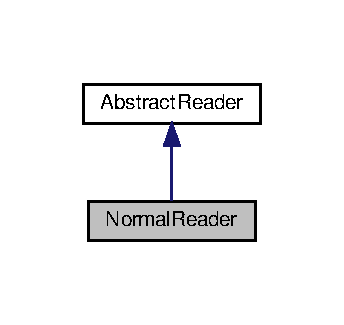
\includegraphics[width=165pt]{classNormalReader__inherit__graph}
\end{center}
\end{figure}


Collaboration diagram for Normal\+Reader\+:\nopagebreak
\begin{figure}[H]
\begin{center}
\leavevmode
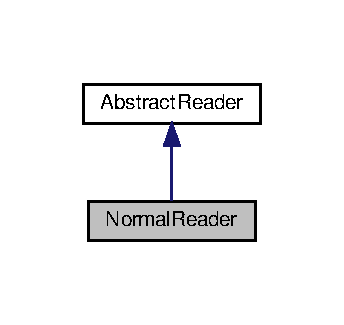
\includegraphics[width=165pt]{classNormalReader__coll__graph}
\end{center}
\end{figure}
\subsection*{Public Member Functions}
\begin{DoxyCompactItemize}
\item 
\mbox{\Hypertarget{classNormalReader_a21910e5b630b535ac9e8a9b55bcb4d06}\label{classNormalReader_a21910e5b630b535ac9e8a9b55bcb4d06}} 
\hyperlink{classNormalReader_a21910e5b630b535ac9e8a9b55bcb4d06}{Normal\+Reader} ()
\begin{DoxyCompactList}\small\item\em \+: Default Constructor \end{DoxyCompactList}\item 
\mbox{\Hypertarget{classNormalReader_a028e517f19b788a043ba170a3bbe24ab}\label{classNormalReader_a028e517f19b788a043ba170a3bbe24ab}} 
\hyperlink{classNormalReader_a028e517f19b788a043ba170a3bbe24ab}{$\sim$\+Normal\+Reader} () override
\begin{DoxyCompactList}\small\item\em \+: Default Destructor \end{DoxyCompactList}\item 
void \hyperlink{classNormalReader_ae6571e3fdc414f143a5541807eded6e0}{read\+\_\+file} (const char $\ast$file, \hyperlink{classAbstractVariable}{Abstract\+Variable} $\ast$\&p\+Random\+Normal) override
\begin{DoxyCompactList}\small\item\em Reads file for distribution type and parameters. \end{DoxyCompactList}\end{DoxyCompactItemize}


\subsection{Detailed Description}
Class to read and store a normal distribution parameters Derived from \hyperlink{classAbstractReader}{Abstract\+Reader}. 

\subsection{Member Function Documentation}
\mbox{\Hypertarget{classNormalReader_ae6571e3fdc414f143a5541807eded6e0}\label{classNormalReader_ae6571e3fdc414f143a5541807eded6e0}} 
\index{Normal\+Reader@{Normal\+Reader}!read\+\_\+file@{read\+\_\+file}}
\index{read\+\_\+file@{read\+\_\+file}!Normal\+Reader@{Normal\+Reader}}
\subsubsection{\texorpdfstring{read\+\_\+file()}{read\_file()}}
{\footnotesize\ttfamily void Normal\+Reader\+::read\+\_\+file (\begin{DoxyParamCaption}\item[{const char $\ast$}]{file,  }\item[{\hyperlink{classAbstractVariable}{Abstract\+Variable} $\ast$\&}]{p\+Random\+Normal }\end{DoxyParamCaption})\hspace{0.3cm}{\ttfamily [override]}, {\ttfamily [virtual]}}



Reads file for distribution type and parameters. 


\begin{DoxyParams}{Parameters}
{\em file} & \+: File name \\
\hline
{\em p\+Random\+Variable} & \+: Pointer to previously to distribution \\
\hline
\end{DoxyParams}


Implements \hyperlink{classAbstractReader_a01d009f3633d0af6d9ea8e34defda7f5}{Abstract\+Reader}.



The documentation for this class was generated from the following files\+:\begin{DoxyCompactItemize}
\item 
Modules/Normal\+Reader.\+h\item 
Modules/Normal\+Reader.\+cpp\end{DoxyCompactItemize}

\hypertarget{structOrderError}{}\section{Order\+Error Struct Reference}
\label{structOrderError}\index{Order\+Error@{Order\+Error}}


Inheritance diagram for Order\+Error\+:\nopagebreak
\begin{figure}[H]
\begin{center}
\leavevmode
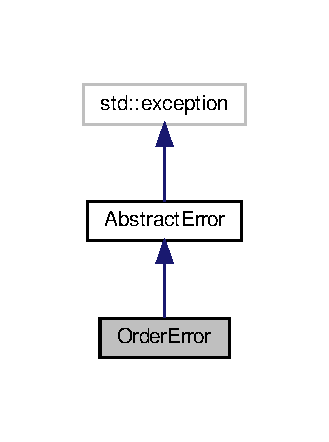
\includegraphics[width=158pt]{structOrderError__inherit__graph}
\end{center}
\end{figure}


Collaboration diagram for Order\+Error\+:\nopagebreak
\begin{figure}[H]
\begin{center}
\leavevmode
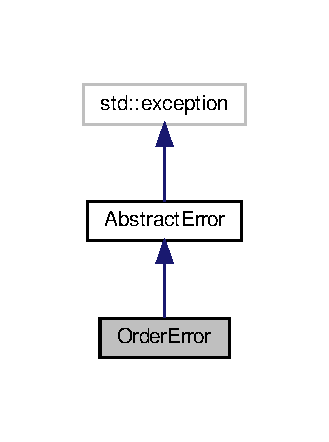
\includegraphics[width=158pt]{structOrderError__coll__graph}
\end{center}
\end{figure}
\subsection*{Public Member Functions}
\begin{DoxyCompactItemize}
\item 
const char $\ast$ \hyperlink{structOrderError_a55140961b8a995ff9111a275cac708c8}{what} () const override  throw ()
\end{DoxyCompactItemize}


\subsection{Member Function Documentation}
\mbox{\Hypertarget{structOrderError_a55140961b8a995ff9111a275cac708c8}\label{structOrderError_a55140961b8a995ff9111a275cac708c8}} 
\index{Order\+Error@{Order\+Error}!what@{what}}
\index{what@{what}!Order\+Error@{Order\+Error}}
\subsubsection{\texorpdfstring{what()}{what()}}
{\footnotesize\ttfamily const char$\ast$ Order\+Error\+::what (\begin{DoxyParamCaption}{ }\end{DoxyParamCaption}) const throw  ) \hspace{0.3cm}{\ttfamily [inline]}, {\ttfamily [override]}, {\ttfamily [virtual]}}

Returns a pointer to the (constant) error description. \begin{DoxyReturn}{Returns}
A pointer to a const char$\ast$. The underlying memory is in possession of the \hyperlink{classAbstractError}{Abstract\+Error} object. Callers must not attempt to free the memory. 
\end{DoxyReturn}


Reimplemented from \hyperlink{classAbstractError_a19735c7a9b5f6e84db606292967667a9}{Abstract\+Error}.



The documentation for this struct was generated from the following file\+:\begin{DoxyCompactItemize}
\item 
Modules/Abstract\+Error.\+h\end{DoxyCompactItemize}

\hypertarget{classPolynomFunc}{}\section{Polynom\+Func Class Reference}
\label{classPolynomFunc}\index{Polynom\+Func@{Polynom\+Func}}


Polynomial function class Derived from \hyperlink{classAbstractFunc}{Abstract\+Func}.  




{\ttfamily \#include $<$Polynom\+Func.\+h$>$}



Inheritance diagram for Polynom\+Func\+:\nopagebreak
\begin{figure}[H]
\begin{center}
\leavevmode
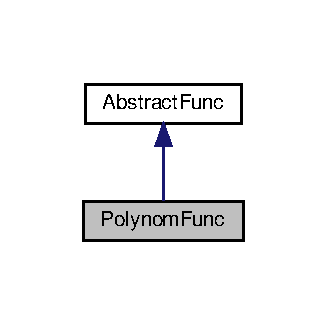
\includegraphics[width=157pt]{classPolynomFunc__inherit__graph}
\end{center}
\end{figure}


Collaboration diagram for Polynom\+Func\+:\nopagebreak
\begin{figure}[H]
\begin{center}
\leavevmode
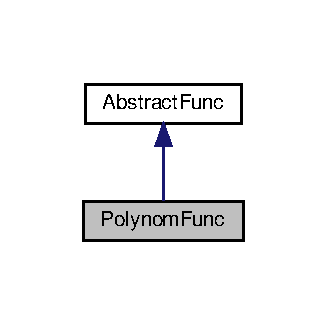
\includegraphics[width=157pt]{classPolynomFunc__coll__graph}
\end{center}
\end{figure}
\subsection*{Public Member Functions}
\begin{DoxyCompactItemize}
\item 
\mbox{\Hypertarget{classPolynomFunc_a49ac41ced1a0d6479edf44edbe086312}\label{classPolynomFunc_a49ac41ced1a0d6479edf44edbe086312}} 
\hyperlink{classPolynomFunc_a49ac41ced1a0d6479edf44edbe086312}{Polynom\+Func} ()
\begin{DoxyCompactList}\small\item\em Default Constructor. \end{DoxyCompactList}\item 
\mbox{\Hypertarget{classPolynomFunc_aed277f31c0410e877a10b5f7298e281c}\label{classPolynomFunc_aed277f31c0410e877a10b5f7298e281c}} 
\hyperlink{classPolynomFunc_aed277f31c0410e877a10b5f7298e281c}{$\sim$\+Polynom\+Func} () override
\begin{DoxyCompactList}\small\item\em Default Destructor. \end{DoxyCompactList}\item 
\hyperlink{classPolynomFunc_a8711146c4bb599be120c35b8404029a9}{Polynom\+Func} (int a, int b)
\begin{DoxyCompactList}\small\item\em Constructor Define the function \char`\"{}ax+b\char`\"{}. \end{DoxyCompactList}\item 
double \hyperlink{classPolynomFunc_a9908fc0cf0686123a98d3186d481fa6f}{evaluate} (double x)
\begin{DoxyCompactList}\small\item\em Return the evaluation of the user polynomial function on a random number. \end{DoxyCompactList}\end{DoxyCompactItemize}
\subsection*{Additional Inherited Members}


\subsection{Detailed Description}
Polynomial function class Derived from \hyperlink{classAbstractFunc}{Abstract\+Func}. 

\subsection{Constructor \& Destructor Documentation}
\mbox{\Hypertarget{classPolynomFunc_a8711146c4bb599be120c35b8404029a9}\label{classPolynomFunc_a8711146c4bb599be120c35b8404029a9}} 
\index{Polynom\+Func@{Polynom\+Func}!Polynom\+Func@{Polynom\+Func}}
\index{Polynom\+Func@{Polynom\+Func}!Polynom\+Func@{Polynom\+Func}}
\subsubsection{\texorpdfstring{Polynom\+Func()}{PolynomFunc()}}
{\footnotesize\ttfamily Polynom\+Func\+::\+Polynom\+Func (\begin{DoxyParamCaption}\item[{int}]{a,  }\item[{int}]{b }\end{DoxyParamCaption})\hspace{0.3cm}{\ttfamily [inline]}}



Constructor Define the function \char`\"{}ax+b\char`\"{}. 


\begin{DoxyParams}{Parameters}
{\em a} & \+: First Coefficient \\
\hline
{\em b} & \+: Second Coefficient \\
\hline
\end{DoxyParams}


\subsection{Member Function Documentation}
\mbox{\Hypertarget{classPolynomFunc_a9908fc0cf0686123a98d3186d481fa6f}\label{classPolynomFunc_a9908fc0cf0686123a98d3186d481fa6f}} 
\index{Polynom\+Func@{Polynom\+Func}!evaluate@{evaluate}}
\index{evaluate@{evaluate}!Polynom\+Func@{Polynom\+Func}}
\subsubsection{\texorpdfstring{evaluate()}{evaluate()}}
{\footnotesize\ttfamily double Polynom\+Func\+::evaluate (\begin{DoxyParamCaption}\item[{double}]{x }\end{DoxyParamCaption})\hspace{0.3cm}{\ttfamily [virtual]}}



Return the evaluation of the user polynomial function on a random number. 


\begin{DoxyParams}{Parameters}
{\em x} & \+: a Random sample \\
\hline
\end{DoxyParams}
\begin{DoxyReturn}{Returns}
a$\ast$x+b 
\end{DoxyReturn}


Implements \hyperlink{classAbstractFunc_ac98be1daa5131b9fddcfdba0a2c34871}{Abstract\+Func}.



The documentation for this class was generated from the following files\+:\begin{DoxyCompactItemize}
\item 
Modules/Polynom\+Func.\+h\item 
Modules/Polynom\+Func.\+cpp\end{DoxyCompactItemize}

\hypertarget{classStatisticalMoment}{}\section{Statistical\+Moment Class Reference}
\label{classStatisticalMoment}\index{Statistical\+Moment@{Statistical\+Moment}}


Class to compute the statistical moments of a given sample.  




{\ttfamily \#include $<$Statistical\+Moment.\+h$>$}

\subsection*{Public Member Functions}
\begin{DoxyCompactItemize}
\item 
\mbox{\Hypertarget{classStatisticalMoment_a7f8b1aac6a3740091045e20dcc68fa51}\label{classStatisticalMoment_a7f8b1aac6a3740091045e20dcc68fa51}} 
\hyperlink{classStatisticalMoment_a7f8b1aac6a3740091045e20dcc68fa51}{Statistical\+Moment} ()
\begin{DoxyCompactList}\small\item\em \+: Default Constructor \end{DoxyCompactList}\item 
\hyperlink{classStatisticalMoment_a31fd5717c856681fc9535837e82fcfbe}{Statistical\+Moment} (\hyperlink{classAbstractVariable}{Abstract\+Variable} $\ast$p\+Random)
\begin{DoxyCompactList}\small\item\em Constructor Define the function \char`\"{}a\+Cos(bx)\char`\"{}. \end{DoxyCompactList}\item 
void \hyperlink{classStatisticalMoment_a7e0fb1cf645bfd8cda912d78c1aa20ed}{write\+\_\+csv} (const char $\ast$file, int order)
\begin{DoxyCompactList}\small\item\em Writes statistical moment to a csv file depending on a given order. \end{DoxyCompactList}\end{DoxyCompactItemize}


\subsection{Detailed Description}
Class to compute the statistical moments of a given sample. 

\subsection{Constructor \& Destructor Documentation}
\mbox{\Hypertarget{classStatisticalMoment_a31fd5717c856681fc9535837e82fcfbe}\label{classStatisticalMoment_a31fd5717c856681fc9535837e82fcfbe}} 
\index{Statistical\+Moment@{Statistical\+Moment}!Statistical\+Moment@{Statistical\+Moment}}
\index{Statistical\+Moment@{Statistical\+Moment}!Statistical\+Moment@{Statistical\+Moment}}
\subsubsection{\texorpdfstring{Statistical\+Moment()}{StatisticalMoment()}}
{\footnotesize\ttfamily Statistical\+Moment\+::\+Statistical\+Moment (\begin{DoxyParamCaption}\item[{\hyperlink{classAbstractVariable}{Abstract\+Variable} $\ast$}]{p\+Random }\end{DoxyParamCaption})}



Constructor Define the function \char`\"{}a\+Cos(bx)\char`\"{}. 


\begin{DoxyParams}{Parameters}
{\em p\+Random} & \\
\hline
\end{DoxyParams}


\subsection{Member Function Documentation}
\mbox{\Hypertarget{classStatisticalMoment_a7e0fb1cf645bfd8cda912d78c1aa20ed}\label{classStatisticalMoment_a7e0fb1cf645bfd8cda912d78c1aa20ed}} 
\index{Statistical\+Moment@{Statistical\+Moment}!write\+\_\+csv@{write\+\_\+csv}}
\index{write\+\_\+csv@{write\+\_\+csv}!Statistical\+Moment@{Statistical\+Moment}}
\subsubsection{\texorpdfstring{write\+\_\+csv()}{write\_csv()}}
{\footnotesize\ttfamily void Statistical\+Moment\+::write\+\_\+csv (\begin{DoxyParamCaption}\item[{const char $\ast$}]{file,  }\item[{int}]{order }\end{DoxyParamCaption})}



Writes statistical moment to a csv file depending on a given order. 


\begin{DoxyParams}{Parameters}
{\em file} & \+: String containing the file name to write the statistical moment to. \\
\hline
{\em order} & \+: Positive Integer that defines statistical order \\
\hline
\end{DoxyParams}


The documentation for this class was generated from the following files\+:\begin{DoxyCompactItemize}
\item 
Modules/Statistical\+Moment.\+h\item 
Modules/Statistical\+Moment.\+cpp\end{DoxyCompactItemize}

\hypertarget{classTrigoFunc}{}\section{Trigo\+Func Class Reference}
\label{classTrigoFunc}\index{Trigo\+Func@{Trigo\+Func}}


Trigonometric function class Derived from \hyperlink{classAbstractFunc}{Abstract\+Func}.  




{\ttfamily \#include $<$Trigo\+Func.\+h$>$}



Inheritance diagram for Trigo\+Func\+:\nopagebreak
\begin{figure}[H]
\begin{center}
\leavevmode
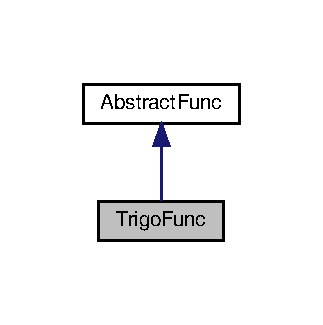
\includegraphics[width=155pt]{classTrigoFunc__inherit__graph}
\end{center}
\end{figure}


Collaboration diagram for Trigo\+Func\+:\nopagebreak
\begin{figure}[H]
\begin{center}
\leavevmode
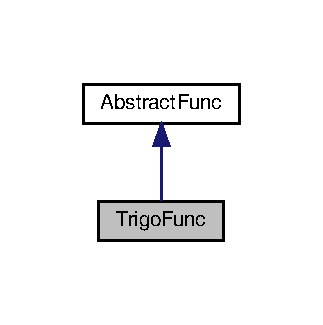
\includegraphics[width=155pt]{classTrigoFunc__coll__graph}
\end{center}
\end{figure}
\subsection*{Public Member Functions}
\begin{DoxyCompactItemize}
\item 
\mbox{\Hypertarget{classTrigoFunc_ad9c2c47ce62daefcbb8c6c0c9d19e227}\label{classTrigoFunc_ad9c2c47ce62daefcbb8c6c0c9d19e227}} 
\hyperlink{classTrigoFunc_ad9c2c47ce62daefcbb8c6c0c9d19e227}{Trigo\+Func} ()
\begin{DoxyCompactList}\small\item\em \+: Default Constructor \end{DoxyCompactList}\item 
\mbox{\Hypertarget{classTrigoFunc_ab29276e57f968adfe36184e4b21f0b37}\label{classTrigoFunc_ab29276e57f968adfe36184e4b21f0b37}} 
\hyperlink{classTrigoFunc_ab29276e57f968adfe36184e4b21f0b37}{$\sim$\+Trigo\+Func} () override
\begin{DoxyCompactList}\small\item\em \+: Default Destructor \end{DoxyCompactList}\item 
\hyperlink{classTrigoFunc_aee28a8cc4b96ef97e3da805b0d9e624e}{Trigo\+Func} (int a, int b)
\begin{DoxyCompactList}\small\item\em Constructor Define the function \char`\"{}a\+Cos(bx)\char`\"{}. \end{DoxyCompactList}\item 
double \hyperlink{classTrigoFunc_ac04acbf2d2b7301d6e2084c9bb8daab2}{evaluate} (double x) override
\begin{DoxyCompactList}\small\item\em Return the evaluation of the user exponential function on a random number. \end{DoxyCompactList}\end{DoxyCompactItemize}
\subsection*{Additional Inherited Members}


\subsection{Detailed Description}
Trigonometric function class Derived from \hyperlink{classAbstractFunc}{Abstract\+Func}. 

\subsection{Constructor \& Destructor Documentation}
\mbox{\Hypertarget{classTrigoFunc_aee28a8cc4b96ef97e3da805b0d9e624e}\label{classTrigoFunc_aee28a8cc4b96ef97e3da805b0d9e624e}} 
\index{Trigo\+Func@{Trigo\+Func}!Trigo\+Func@{Trigo\+Func}}
\index{Trigo\+Func@{Trigo\+Func}!Trigo\+Func@{Trigo\+Func}}
\subsubsection{\texorpdfstring{Trigo\+Func()}{TrigoFunc()}}
{\footnotesize\ttfamily Trigo\+Func\+::\+Trigo\+Func (\begin{DoxyParamCaption}\item[{int}]{a,  }\item[{int}]{b }\end{DoxyParamCaption})\hspace{0.3cm}{\ttfamily [inline]}}



Constructor Define the function \char`\"{}a\+Cos(bx)\char`\"{}. 


\begin{DoxyParams}{Parameters}
{\em a} & First Coefficient \\
\hline
{\em b} & Second Coefficient \\
\hline
\end{DoxyParams}


\subsection{Member Function Documentation}
\mbox{\Hypertarget{classTrigoFunc_ac04acbf2d2b7301d6e2084c9bb8daab2}\label{classTrigoFunc_ac04acbf2d2b7301d6e2084c9bb8daab2}} 
\index{Trigo\+Func@{Trigo\+Func}!evaluate@{evaluate}}
\index{evaluate@{evaluate}!Trigo\+Func@{Trigo\+Func}}
\subsubsection{\texorpdfstring{evaluate()}{evaluate()}}
{\footnotesize\ttfamily double Trigo\+Func\+::evaluate (\begin{DoxyParamCaption}\item[{double}]{x }\end{DoxyParamCaption})\hspace{0.3cm}{\ttfamily [override]}, {\ttfamily [virtual]}}



Return the evaluation of the user exponential function on a random number. 


\begin{DoxyParams}{Parameters}
{\em x} & \+: a Random number \\
\hline
\end{DoxyParams}
\begin{DoxyReturn}{Returns}
a$\ast$\+Cos(bx) 
\end{DoxyReturn}


Implements \hyperlink{classAbstractFunc_ac98be1daa5131b9fddcfdba0a2c34871}{Abstract\+Func}.



The documentation for this class was generated from the following files\+:\begin{DoxyCompactItemize}
\item 
Modules/Trigo\+Func.\+h\item 
Modules/Trigo\+Func.\+cpp\end{DoxyCompactItemize}

\hypertarget{classUniformDist}{}\section{Uniform\+Dist Class Reference}
\label{classUniformDist}\index{Uniform\+Dist@{Uniform\+Dist}}


Class to create an uniform distribution sample using random generator Derived from Abstract Variable class.  




{\ttfamily \#include $<$Uniform\+Dist.\+h$>$}



Inheritance diagram for Uniform\+Dist\+:\nopagebreak
\begin{figure}[H]
\begin{center}
\leavevmode
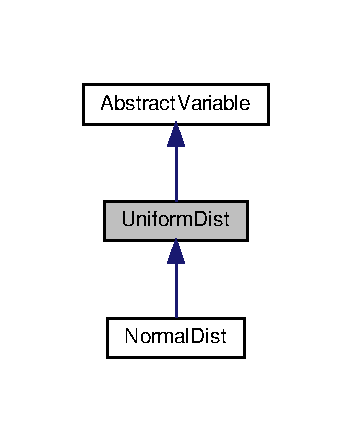
\includegraphics[width=169pt]{classUniformDist__inherit__graph}
\end{center}
\end{figure}


Collaboration diagram for Uniform\+Dist\+:\nopagebreak
\begin{figure}[H]
\begin{center}
\leavevmode
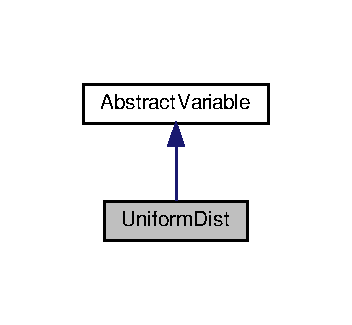
\includegraphics[width=169pt]{classUniformDist__coll__graph}
\end{center}
\end{figure}
\subsection*{Public Member Functions}
\begin{DoxyCompactItemize}
\item 
\mbox{\Hypertarget{classUniformDist_aff015d27dc0cd334fa189e9a69df890b}\label{classUniformDist_aff015d27dc0cd334fa189e9a69df890b}} 
\hyperlink{classUniformDist_aff015d27dc0cd334fa189e9a69df890b}{Uniform\+Dist} ()
\begin{DoxyCompactList}\small\item\em Default Constructor. \end{DoxyCompactList}\item 
\hyperlink{classUniformDist_a723002562ed94ff786c30048268609cb}{Uniform\+Dist} (const int N)
\begin{DoxyCompactList}\small\item\em Constructor. \end{DoxyCompactList}\item 
\hyperlink{classUniformDist_ade2ddd82d83472112ce24c575880134d}{Uniform\+Dist} (const int N, const int a, const int b)
\begin{DoxyCompactList}\small\item\em Constructor Compute a sample from the standard uniform distribution of lower bound a and high bound b. \end{DoxyCompactList}\item 
virtual std\+::vector$<$ double $>$ \hyperlink{classUniformDist_a60df487bfb003628e9997ebcb5aedcde}{get\+\_\+vector} () const
\begin{DoxyCompactList}\small\item\em Return the vector of the normal sample. \end{DoxyCompactList}\item 
virtual double \hyperlink{classUniformDist_a18371ef0295e7aca4085015c0d844b41}{get\+\_\+mean} () const
\begin{DoxyCompactList}\small\item\em Return the mean of the normal sample. \end{DoxyCompactList}\item 
virtual double \hyperlink{classUniformDist_aade143a6ff9ed9a8bee2e6b9fb2fed4c}{get\+\_\+var} () const
\begin{DoxyCompactList}\small\item\em Return the variance of the normal sample. \end{DoxyCompactList}\item 
virtual int \hyperlink{classUniformDist_a6e7a871053b2eb563fcbf2f7e02fb22b}{get\+\_\+size} () const
\begin{DoxyCompactList}\small\item\em Return the length of the normal sample. \end{DoxyCompactList}\end{DoxyCompactItemize}
\subsection*{Protected Attributes}
\begin{DoxyCompactItemize}
\item 
\mbox{\Hypertarget{classUniformDist_addefdf54211e913830006e833a192748}\label{classUniformDist_addefdf54211e913830006e833a192748}} 
std\+::vector$<$ double $>$ {\bfseries uniform\+Samples}
\end{DoxyCompactItemize}


\subsection{Detailed Description}
Class to create an uniform distribution sample using random generator Derived from Abstract Variable class. 

\subsection{Constructor \& Destructor Documentation}
\mbox{\Hypertarget{classUniformDist_a723002562ed94ff786c30048268609cb}\label{classUniformDist_a723002562ed94ff786c30048268609cb}} 
\index{Uniform\+Dist@{Uniform\+Dist}!Uniform\+Dist@{Uniform\+Dist}}
\index{Uniform\+Dist@{Uniform\+Dist}!Uniform\+Dist@{Uniform\+Dist}}
\subsubsection{\texorpdfstring{Uniform\+Dist()}{UniformDist()}\hspace{0.1cm}{\footnotesize\ttfamily [1/2]}}
{\footnotesize\ttfamily Uniform\+Dist\+::\+Uniform\+Dist (\begin{DoxyParamCaption}\item[{const int}]{N }\end{DoxyParamCaption})}



Constructor. 


\begin{DoxyParams}{Parameters}
{\em N} & \\
\hline
\end{DoxyParams}
\mbox{\Hypertarget{classUniformDist_ade2ddd82d83472112ce24c575880134d}\label{classUniformDist_ade2ddd82d83472112ce24c575880134d}} 
\index{Uniform\+Dist@{Uniform\+Dist}!Uniform\+Dist@{Uniform\+Dist}}
\index{Uniform\+Dist@{Uniform\+Dist}!Uniform\+Dist@{Uniform\+Dist}}
\subsubsection{\texorpdfstring{Uniform\+Dist()}{UniformDist()}\hspace{0.1cm}{\footnotesize\ttfamily [2/2]}}
{\footnotesize\ttfamily Uniform\+Dist\+::\+Uniform\+Dist (\begin{DoxyParamCaption}\item[{const int}]{N,  }\item[{const int}]{a,  }\item[{const int}]{b }\end{DoxyParamCaption})}



Constructor Compute a sample from the standard uniform distribution of lower bound a and high bound b. 


\begin{DoxyParams}{Parameters}
{\em N} & \+: Positive integer defining sample size \\
\hline
{\em a} & \+: Integer for lower bound \\
\hline
{\em b} & \+: Integer for higher bound \\
\hline
\end{DoxyParams}


\subsection{Member Function Documentation}
\mbox{\Hypertarget{classUniformDist_a18371ef0295e7aca4085015c0d844b41}\label{classUniformDist_a18371ef0295e7aca4085015c0d844b41}} 
\index{Uniform\+Dist@{Uniform\+Dist}!get\+\_\+mean@{get\+\_\+mean}}
\index{get\+\_\+mean@{get\+\_\+mean}!Uniform\+Dist@{Uniform\+Dist}}
\subsubsection{\texorpdfstring{get\+\_\+mean()}{get\_mean()}}
{\footnotesize\ttfamily virtual double Uniform\+Dist\+::get\+\_\+mean (\begin{DoxyParamCaption}{ }\end{DoxyParamCaption}) const\hspace{0.3cm}{\ttfamily [inline]}, {\ttfamily [virtual]}}



Return the mean of the normal sample. 

\begin{DoxyReturn}{Returns}
the mean of the normal sample. 
\end{DoxyReturn}


Implements \hyperlink{classAbstractVariable_a99ceeeecc689a9683badfdfa7ef20c45}{Abstract\+Variable}.



Reimplemented in \hyperlink{classNormalDist_a947707f47873251fd7857b4a7ed977bc}{Normal\+Dist}.

\mbox{\Hypertarget{classUniformDist_a6e7a871053b2eb563fcbf2f7e02fb22b}\label{classUniformDist_a6e7a871053b2eb563fcbf2f7e02fb22b}} 
\index{Uniform\+Dist@{Uniform\+Dist}!get\+\_\+size@{get\+\_\+size}}
\index{get\+\_\+size@{get\+\_\+size}!Uniform\+Dist@{Uniform\+Dist}}
\subsubsection{\texorpdfstring{get\+\_\+size()}{get\_size()}}
{\footnotesize\ttfamily virtual int Uniform\+Dist\+::get\+\_\+size (\begin{DoxyParamCaption}{ }\end{DoxyParamCaption}) const\hspace{0.3cm}{\ttfamily [inline]}, {\ttfamily [virtual]}}



Return the length of the normal sample. 

\begin{DoxyReturn}{Returns}
The length of the normal sample 
\end{DoxyReturn}


Implements \hyperlink{classAbstractVariable_a96d9b63c3d9aff4673a9c66738302766}{Abstract\+Variable}.



Reimplemented in \hyperlink{classNormalDist_a6dcfba2a8149dbd527392c32b3d7a7a1}{Normal\+Dist}.

\mbox{\Hypertarget{classUniformDist_aade143a6ff9ed9a8bee2e6b9fb2fed4c}\label{classUniformDist_aade143a6ff9ed9a8bee2e6b9fb2fed4c}} 
\index{Uniform\+Dist@{Uniform\+Dist}!get\+\_\+var@{get\+\_\+var}}
\index{get\+\_\+var@{get\+\_\+var}!Uniform\+Dist@{Uniform\+Dist}}
\subsubsection{\texorpdfstring{get\+\_\+var()}{get\_var()}}
{\footnotesize\ttfamily virtual double Uniform\+Dist\+::get\+\_\+var (\begin{DoxyParamCaption}{ }\end{DoxyParamCaption}) const\hspace{0.3cm}{\ttfamily [inline]}, {\ttfamily [virtual]}}



Return the variance of the normal sample. 

\begin{DoxyReturn}{Returns}
the variance of the normal sample 
\end{DoxyReturn}


Implements \hyperlink{classAbstractVariable_a71d378332b0e5b3c1760bb98db5d906b}{Abstract\+Variable}.



Reimplemented in \hyperlink{classNormalDist_a46bc646f126ac3c2d46bcd9ccbf01135}{Normal\+Dist}.

\mbox{\Hypertarget{classUniformDist_a60df487bfb003628e9997ebcb5aedcde}\label{classUniformDist_a60df487bfb003628e9997ebcb5aedcde}} 
\index{Uniform\+Dist@{Uniform\+Dist}!get\+\_\+vector@{get\+\_\+vector}}
\index{get\+\_\+vector@{get\+\_\+vector}!Uniform\+Dist@{Uniform\+Dist}}
\subsubsection{\texorpdfstring{get\+\_\+vector()}{get\_vector()}}
{\footnotesize\ttfamily virtual std\+::vector$<$double$>$ Uniform\+Dist\+::get\+\_\+vector (\begin{DoxyParamCaption}{ }\end{DoxyParamCaption}) const\hspace{0.3cm}{\ttfamily [inline]}, {\ttfamily [virtual]}}



Return the vector of the normal sample. 

\begin{DoxyReturn}{Returns}
the vector of the sample 
\end{DoxyReturn}


Implements \hyperlink{classAbstractVariable_a0312a988d8c527d2af7615ef2fd08621}{Abstract\+Variable}.



Reimplemented in \hyperlink{classNormalDist_a473e67b9d1787f6ff887f6854dbd350c}{Normal\+Dist}.



The documentation for this class was generated from the following files\+:\begin{DoxyCompactItemize}
\item 
Modules/Uniform\+Dist.\+h\item 
Modules/Uniform\+Dist.\+cpp\end{DoxyCompactItemize}

\hypertarget{classUniformReader}{}\section{Uniform\+Reader Class Reference}
\label{classUniformReader}\index{Uniform\+Reader@{Uniform\+Reader}}


Class to read and store a uniform distribution parameters Derived from \hyperlink{classAbstractReader}{Abstract\+Reader}.  




{\ttfamily \#include $<$Uniform\+Reader.\+h$>$}



Inheritance diagram for Uniform\+Reader\+:\nopagebreak
\begin{figure}[H]
\begin{center}
\leavevmode
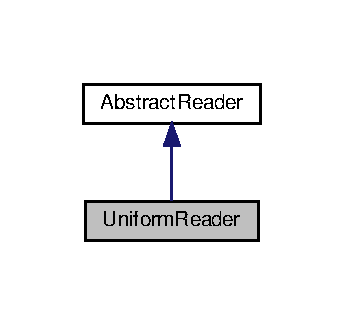
\includegraphics[width=165pt]{classUniformReader__inherit__graph}
\end{center}
\end{figure}


Collaboration diagram for Uniform\+Reader\+:\nopagebreak
\begin{figure}[H]
\begin{center}
\leavevmode
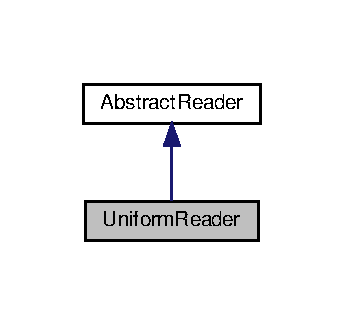
\includegraphics[width=165pt]{classUniformReader__coll__graph}
\end{center}
\end{figure}
\subsection*{Public Member Functions}
\begin{DoxyCompactItemize}
\item 
\mbox{\Hypertarget{classUniformReader_ac6ba86e0db2e3dfe4c5204295c78c5a9}\label{classUniformReader_ac6ba86e0db2e3dfe4c5204295c78c5a9}} 
\hyperlink{classUniformReader_ac6ba86e0db2e3dfe4c5204295c78c5a9}{Uniform\+Reader} ()
\begin{DoxyCompactList}\small\item\em Default Constructor. \end{DoxyCompactList}\item 
\mbox{\Hypertarget{classUniformReader_a4e6558861df3bb2c14670c2b7cd46758}\label{classUniformReader_a4e6558861df3bb2c14670c2b7cd46758}} 
\hyperlink{classUniformReader_a4e6558861df3bb2c14670c2b7cd46758}{$\sim$\+Uniform\+Reader} () override
\begin{DoxyCompactList}\small\item\em Default Destructor. \end{DoxyCompactList}\item 
void \hyperlink{classUniformReader_ae4e326a00cd72cdc1afa73beebe60ddc}{read\+\_\+file} (const char $\ast$file, \hyperlink{classAbstractVariable}{Abstract\+Variable} $\ast$\&p\+Random\+Variable) override
\begin{DoxyCompactList}\small\item\em Reads file for distribution type and parameters. \end{DoxyCompactList}\end{DoxyCompactItemize}


\subsection{Detailed Description}
Class to read and store a uniform distribution parameters Derived from \hyperlink{classAbstractReader}{Abstract\+Reader}. 

\subsection{Member Function Documentation}
\mbox{\Hypertarget{classUniformReader_ae4e326a00cd72cdc1afa73beebe60ddc}\label{classUniformReader_ae4e326a00cd72cdc1afa73beebe60ddc}} 
\index{Uniform\+Reader@{Uniform\+Reader}!read\+\_\+file@{read\+\_\+file}}
\index{read\+\_\+file@{read\+\_\+file}!Uniform\+Reader@{Uniform\+Reader}}
\subsubsection{\texorpdfstring{read\+\_\+file()}{read\_file()}}
{\footnotesize\ttfamily void Uniform\+Reader\+::read\+\_\+file (\begin{DoxyParamCaption}\item[{const char $\ast$}]{file,  }\item[{\hyperlink{classAbstractVariable}{Abstract\+Variable} $\ast$\&}]{p\+Random\+Variable }\end{DoxyParamCaption})\hspace{0.3cm}{\ttfamily [override]}, {\ttfamily [virtual]}}



Reads file for distribution type and parameters. 


\begin{DoxyParams}{Parameters}
{\em file} & \+: File name \\
\hline
{\em p\+Random\+Variable} & \+: Pointer to previously to distribution \\
\hline
\end{DoxyParams}


Implements \hyperlink{classAbstractReader_a01d009f3633d0af6d9ea8e34defda7f5}{Abstract\+Reader}.



The documentation for this class was generated from the following files\+:\begin{DoxyCompactItemize}
\item 
Modules/Uniform\+Reader.\+h\item 
Modules/Uniform\+Reader.\+cpp\end{DoxyCompactItemize}

\hypertarget{structVarError}{}\section{Var\+Error Struct Reference}
\label{structVarError}\index{Var\+Error@{Var\+Error}}


Inheritance diagram for Var\+Error\+:\nopagebreak
\begin{figure}[H]
\begin{center}
\leavevmode
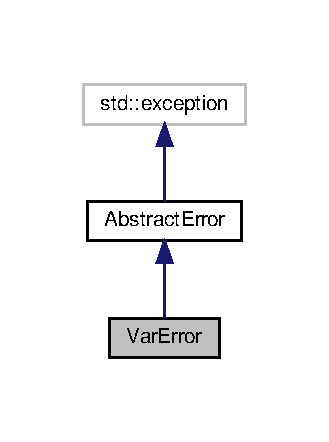
\includegraphics[width=158pt]{structVarError__inherit__graph}
\end{center}
\end{figure}


Collaboration diagram for Var\+Error\+:\nopagebreak
\begin{figure}[H]
\begin{center}
\leavevmode
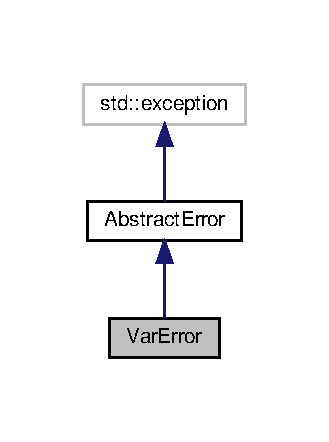
\includegraphics[width=158pt]{structVarError__coll__graph}
\end{center}
\end{figure}
\subsection*{Public Member Functions}
\begin{DoxyCompactItemize}
\item 
const char $\ast$ \hyperlink{structVarError_a48ee904c5e61633cb6f4b9af2d093eaa}{what} () const override  throw ()
\end{DoxyCompactItemize}


\subsection{Member Function Documentation}
\mbox{\Hypertarget{structVarError_a48ee904c5e61633cb6f4b9af2d093eaa}\label{structVarError_a48ee904c5e61633cb6f4b9af2d093eaa}} 
\index{Var\+Error@{Var\+Error}!what@{what}}
\index{what@{what}!Var\+Error@{Var\+Error}}
\subsubsection{\texorpdfstring{what()}{what()}}
{\footnotesize\ttfamily const char$\ast$ Var\+Error\+::what (\begin{DoxyParamCaption}{ }\end{DoxyParamCaption}) const throw  ) \hspace{0.3cm}{\ttfamily [inline]}, {\ttfamily [override]}, {\ttfamily [virtual]}}

Returns a pointer to the (constant) error description. \begin{DoxyReturn}{Returns}
A pointer to a const char$\ast$. The underlying memory is in possession of the \hyperlink{classAbstractError}{Abstract\+Error} object. Callers must not attempt to free the memory. 
\end{DoxyReturn}


Reimplemented from \hyperlink{classAbstractError_a19735c7a9b5f6e84db606292967667a9}{Abstract\+Error}.



The documentation for this struct was generated from the following file\+:\begin{DoxyCompactItemize}
\item 
Modules/Abstract\+Error.\+h\end{DoxyCompactItemize}

\hypertarget{structVectSizeError}{}\section{Vect\+Size\+Error Struct Reference}
\label{structVectSizeError}\index{Vect\+Size\+Error@{Vect\+Size\+Error}}


Inheritance diagram for Vect\+Size\+Error\+:\nopagebreak
\begin{figure}[H]
\begin{center}
\leavevmode
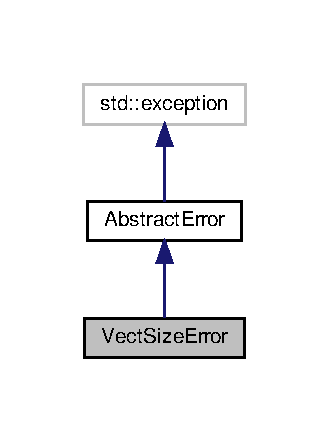
\includegraphics[width=158pt]{structVectSizeError__inherit__graph}
\end{center}
\end{figure}


Collaboration diagram for Vect\+Size\+Error\+:\nopagebreak
\begin{figure}[H]
\begin{center}
\leavevmode
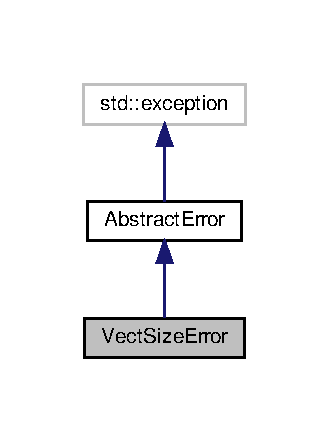
\includegraphics[width=158pt]{structVectSizeError__coll__graph}
\end{center}
\end{figure}
\subsection*{Public Member Functions}
\begin{DoxyCompactItemize}
\item 
const char $\ast$ \hyperlink{structVectSizeError_af92248320a9fb06b025662736a742c9e}{what} () const override  throw ()
\end{DoxyCompactItemize}


\subsection{Member Function Documentation}
\mbox{\Hypertarget{structVectSizeError_af92248320a9fb06b025662736a742c9e}\label{structVectSizeError_af92248320a9fb06b025662736a742c9e}} 
\index{Vect\+Size\+Error@{Vect\+Size\+Error}!what@{what}}
\index{what@{what}!Vect\+Size\+Error@{Vect\+Size\+Error}}
\subsubsection{\texorpdfstring{what()}{what()}}
{\footnotesize\ttfamily const char$\ast$ Vect\+Size\+Error\+::what (\begin{DoxyParamCaption}{ }\end{DoxyParamCaption}) const throw  ) \hspace{0.3cm}{\ttfamily [inline]}, {\ttfamily [override]}, {\ttfamily [virtual]}}

Returns a pointer to the (constant) error description. \begin{DoxyReturn}{Returns}
A pointer to a const char$\ast$. The underlying memory is in possession of the \hyperlink{classAbstractError}{Abstract\+Error} object. Callers must not attempt to free the memory. 
\end{DoxyReturn}


Reimplemented from \hyperlink{classAbstractError_a19735c7a9b5f6e84db606292967667a9}{Abstract\+Error}.



The documentation for this struct was generated from the following file\+:\begin{DoxyCompactItemize}
\item 
Modules/Abstract\+Error.\+h\end{DoxyCompactItemize}

\hypertarget{structWrongFormatError}{}\section{Wrong\+Format\+Error Struct Reference}
\label{structWrongFormatError}\index{Wrong\+Format\+Error@{Wrong\+Format\+Error}}


Inheritance diagram for Wrong\+Format\+Error\+:\nopagebreak
\begin{figure}[H]
\begin{center}
\leavevmode
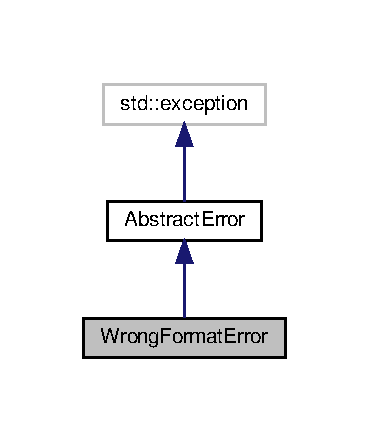
\includegraphics[width=177pt]{structWrongFormatError__inherit__graph}
\end{center}
\end{figure}


Collaboration diagram for Wrong\+Format\+Error\+:\nopagebreak
\begin{figure}[H]
\begin{center}
\leavevmode
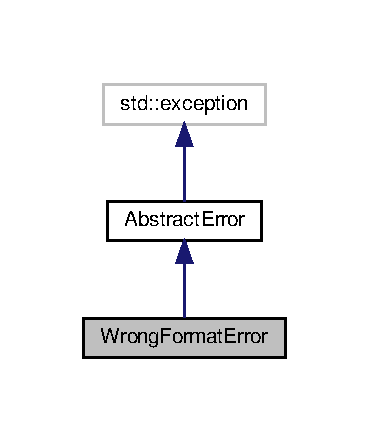
\includegraphics[width=177pt]{structWrongFormatError__coll__graph}
\end{center}
\end{figure}
\subsection*{Public Member Functions}
\begin{DoxyCompactItemize}
\item 
const char $\ast$ \hyperlink{structWrongFormatError_a3c1c3f39ce135d19c7d0bb2fe8ddd3c1}{what} () const override  throw ()
\end{DoxyCompactItemize}


\subsection{Member Function Documentation}
\mbox{\Hypertarget{structWrongFormatError_a3c1c3f39ce135d19c7d0bb2fe8ddd3c1}\label{structWrongFormatError_a3c1c3f39ce135d19c7d0bb2fe8ddd3c1}} 
\index{Wrong\+Format\+Error@{Wrong\+Format\+Error}!what@{what}}
\index{what@{what}!Wrong\+Format\+Error@{Wrong\+Format\+Error}}
\subsubsection{\texorpdfstring{what()}{what()}}
{\footnotesize\ttfamily const char$\ast$ Wrong\+Format\+Error\+::what (\begin{DoxyParamCaption}{ }\end{DoxyParamCaption}) const throw  ) \hspace{0.3cm}{\ttfamily [inline]}, {\ttfamily [override]}, {\ttfamily [virtual]}}

Returns a pointer to the (constant) error description. \begin{DoxyReturn}{Returns}
A pointer to a const char$\ast$. The underlying memory is in possession of the \hyperlink{classAbstractError}{Abstract\+Error} object. Callers must not attempt to free the memory. 
\end{DoxyReturn}


Reimplemented from \hyperlink{classAbstractError_a19735c7a9b5f6e84db606292967667a9}{Abstract\+Error}.



The documentation for this struct was generated from the following file\+:\begin{DoxyCompactItemize}
\item 
Modules/Abstract\+Error.\+h\end{DoxyCompactItemize}

%--- End generated contents ---

% Index
\backmatter
\newpage
\phantomsection
\clearemptydoublepage
\addcontentsline{toc}{chapter}{Index}
\printindex

\end{document}
